%\section{Implementation of the Imaging System}
What is required to select a suitable landing site? What are the main objectives of the Imaging System? How does the physical properties of the orbiter limit the design? The answers to these questions define the initial system requirements for the design.
%\subsection{Selecting a suitable landing site}
\subsection{System Objectives}
To successfully select a landing site, it is necessary to gather more information about the lunar surface of Europa. This objective leads to a set of image system requirements. 
\begin{figure}[htb!]
%left bottom right top
\centering
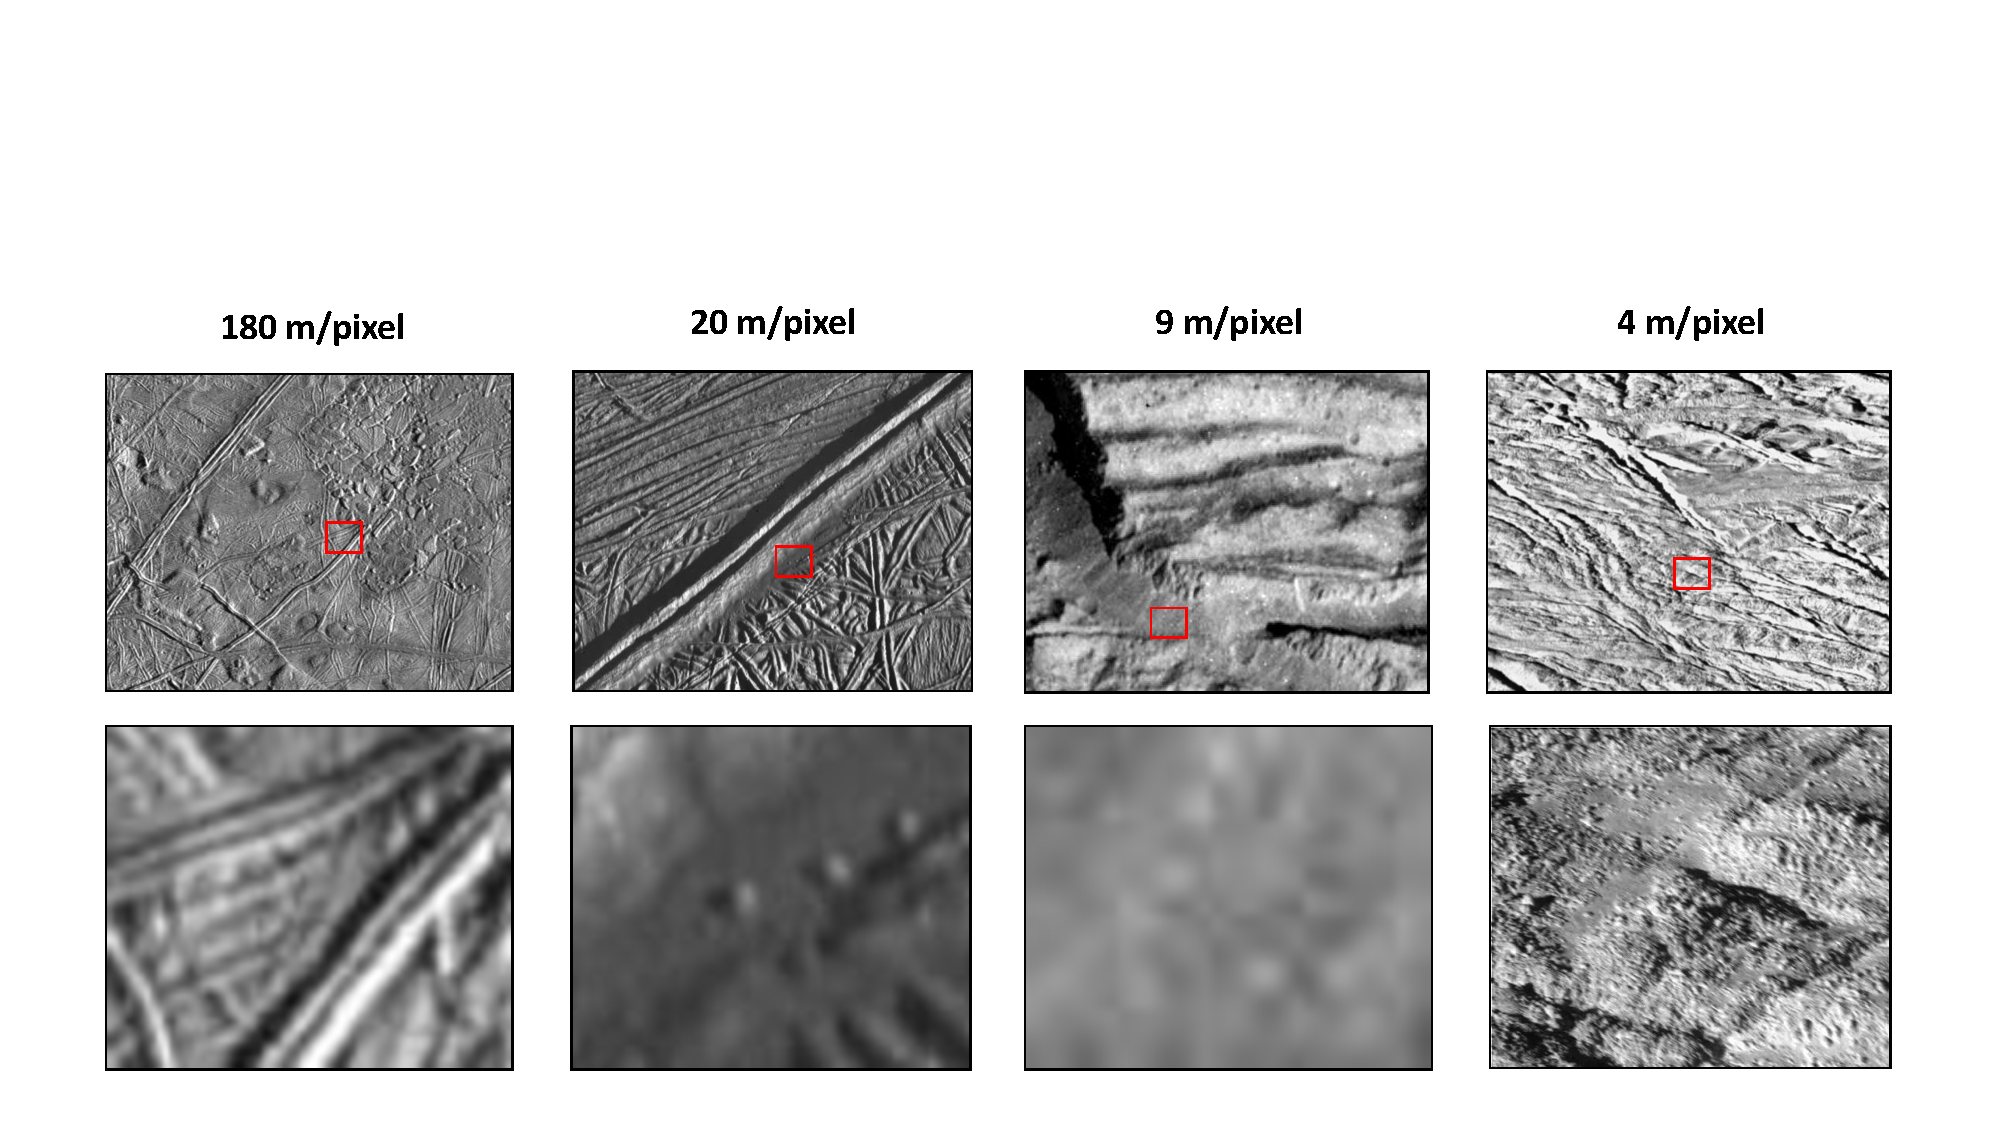
\includegraphics[width=1\textwidth,page=1,trim=10mm 5mm 15mm 50mm,clip]{figures/Orbiter/highres.pdf}
\caption{Ground resolution comparison. Left: three image sets of Europa from Galileo spacecraft Right: Enceladus high resolution taken from the Cassini spacecraft.}
\label{fig:highres_compare}
\end{figure}
\begin{description}
\item[Resolution]
The resolution for the WAC must be high enough that it is possible to identify ROIs. Based on figure (\ref{fig:highres_compare}), a resolution of 100 meters per pixel MPP is expected to be adequate for the worst case resolution, i.e. the resolution at the far operating distance. This defines the requirement for the WAC. The WAC will be producing the low resolution images used for the initial analysis and ROI selection.

When investigating the individual ROIs, it is expected that objects around the size of the lander (and larger) will pose a danger to the lander and must therefore be avoided. Assuming the lander will be around 1 meter in diameter, the smallest feature that must be detected must be 1 meter. Referring to \cite{andor2016}, \cite{ni2014} and \cite{sbig2014}, a minimum of two pixels per smallest feature is necessary, to make an accurate measurement on the image. This defines the required resolution of 0.5 MPP for the NAC.

It is expected that a high enough resolution will make it possible to detect most surface roughness and elevation, based on figure (\ref{fig:highres_compare}). However, if a detailed topographic mapping of the surface is necessary, it may be needed to operate the imaging system in stereo or to use additional instruments. Stereo imaging does not necessarily require two cameras. Instead, the movement of the spacecraft can be used to obtain images from two different angles, resulting in a stereo image. 
\item[Surface Chemistry]
The surface chemistry should be analysed, as some areas on Europa may be unsuitable due to the chemical compounds. One relatively simple way to enhance the imaging system is to add a selection of filters to the imaging system, making it possible to observe the radiance at different wavelengths. Ultimately, a spectra can be created of a given area. The spectra can later be analysed and compared to known chemical compounds or materials. The higher the number of spectral bands, the more accurate the surface can be assessed. This type of enhancement is a good way to enhance an existing system, sharing the existing resources and costs, while providing additional capabilities to the orbiter.
%Adding imaging spectrometer capabilities to the imaging system is one way to enhance an existing system to provide extra functionality, without adding extra instruments.
%make it possible to assess the surface chemistry, while sharing the existing resources. using the capabilities of  without adding extra instruments.
\item[Ice surface Assessment]
In addition to the assessment of the surface chemistry, the ice surface must be analysed. Knowledge about the ice surface should make it possible to select a relatively clean ice surface, with less particles or dust. Since the proposed penetrator relies on melting the ice, inhomogeneous ice may cause the hole to clog with particles, bringing the melting process to a standstill. It is expected that the icy surface will not be homogeneous, based on the analysis in section (\ref{sec:lenticulae}). However, some zones may be dirtier than others, and will be unsuited for a landing site. Being able to differentiate between ice types will be a great help when selecting suitable landing sites. A recent study \cite{naegeli2015a} proposed the use of imaging spectroscopy for assessing the ice surface composition. The results from this study suggests imaging spectroscopy could be a good solution to this problem.
\end{description}
\subsection{Mission Constraints}
The main objectives of the mission to Europa is to look for life. Surveying therefore plays a smaller role in the mission. The majority of the instruments included on the mission will be used to look for life but this does not include the imaging system. Therefore, the mass, volume and power allocated for this system will be constrained.

Without an imaging system on the orbiter, it will not be realistic to land on Europa. The existing images and knowledge about the surface is too limited, expressing the need for additional surveying beforehand. The system is therefore necessary but must be focused on providing mission critical data. It is preferred if the support systems required by the imaging system can be shared with the remaining systems. Without any cost sharing, it is doubtful that the remaining mission teams will be supportive of the imaging system.
\subsection{Orbit Constraints}
The coverage that can be provided by the imaging system will be limited by the choice of orbit. When designing the telescopes and cameras, it is crucial to have knowledge about the working distance of the imaging system. Therefore, the orbits must be planned in detail to ensure adequate coverage can be achieved and that the imaging system will be operating within their suitable ranges.

The choice of orbit will affect the lifetime of the imaging system, as the radiation environment varies greatly. Naturally, this will also affect the required radiation shielding and the mass and volume requirements.
%\todo[inline]{More to add about orbit constraints? Radiation?}
%\subsection{Alignment and Calibration}
%\todo[inline]{Implementation: Include ways to calibrate, align spacecraft/telescope}
%\newpage
\section{System Overview}
Due to the complexity of the imaging system, the system will be split in individual subsystems. For each subsystem, a set of solutions will be proposed. First, the overall structure of the image system will be defined, creating the framework for the proposed imaging system.
\subsection{Imaging System Structure}
When selecting the structure, the first question is the number of cameras that should be provided. Naturally, a single camera will provide a simple design but would also limit the tasks that can be completed by the imaging system. A camera is usually limited to relatively narrow working range and will be designed as either a wide angle camera (WAC) or narrow angle camera (NAC), depending on the required range. The WAC would be very useful for the identification of ROIs. During this phase, a large surface area must be mapped during relatively few flybys. The large field of view (FOV) of the WAC means a large surface area can be covered, but in a low resolution. In contrast, the NAC would be very suitable for the high resolution imaging of interesting regions but would require many flybys to achieve a high enough coverage of the surface.

Mapping and surveying Europa is not the primary goal of the mission but is necessary, before the landing can proceed. Therefore, the allocated resources for the imaging system will not be unlimited. Since the imaging system does not have top priority in this mission, it is important to consider how the system can provide useful data for the remaining groups. Having a WAC is very useful for the orbit determination, as it will be suitable for observing a large planet or satellite together with the background star field, providing the opnav images used for orbit determination. Having both a WAC and a NAC is also very useful for the lander guidance objective and geolocation. The "global" mapping can be provided by the WAC whereas the "local" mapping can be provided by the NAC. By correlating the two image sets, geo-localisation in both high and low resolution is possible.

Tracking a fast moving object with a NAC can be very difficult, as the object can easily move outside the camera frame - causing a loss of tracking. A WAC makes it possible to track the lander, without requiring a high pointing accuracy. As long as the camera is pointing in the general direction of the lander, the lander will remain within the camera frame.

Another important aspect to consider is the redundancy of the camera system. Naturally, having duplicate systems available is preferred, if one system fails. One type of redundancy is to have an identical camera on standby but this will require a larger allocation of resources for a system, that may not be necessary, unless a camera actually fails. A different approach is to bring both a NAC and WAC. While each camera is suited for a specific task, they can substitute each other to a degree, if one camera fails. However, the performance of the image system will be degraded, depending on which camera that fails. The WAC is the most irreplaceable one of the cameras, as it will not be possible to cover a large enough surface area, without this camera. In the event of a WAC failure, many more flybys will be required to obtain adequate coverage - prolonging the mission.

The WAC can operate on its own, but it will require a dynamic flyby to re-target a specific region of interest. After covering the area in low resolution, it will be necessary to cover the area again, using a higher resolution (and therefore a lower altitude). The WAC can only provide an adequate resolution, if the orbiter passes closer to Europa. As an alternative, zoom capabilities can be added to the WAC, to provide higher resolution imaging but this will require a more complex design and moving parts.

When considering camera systems that can provide topographic data about the surface, it is natural to consider stereo imaging. The common way to generate stereo images is to operate two cameras at once, each viewing the scene from a slightly different angle. As this is a costly approach, an alternative way is proposed for this mission. By using the spacecraft attitude control systems to move the spacecraft, it is possible to generate stereo images, using only one camera. This method is illustrated in figure \ref{fig:stereoimg}. Naturally, it will require more from the attitude control systems, as the spacecraft must be able to point in specific directions on command. However, using this approach, stereo imaging can be added - independent on the number of cameras provided by the orbiter.

\begin{figure}[htb!]
\centering
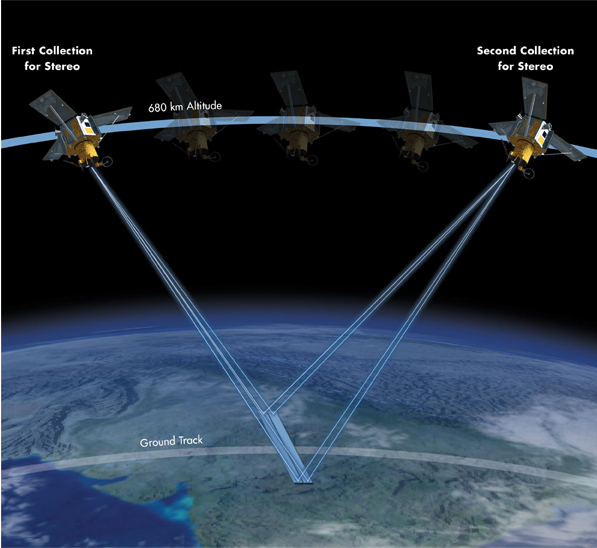
\includegraphics[width=0.4\textwidth]{figures/Orbiter/Stereo_Satellite.png}
\caption{Stereo Imaging using one camera. Source: DigitalGlobe, \cite{satimgcorp2015}.}
\label{fig:stereoimg}
\end{figure}

The two structures are compared in table (\ref{tab:score_system_structure}). It is apparent that the single camera method is a simple and cheap but it will be less suited for a surface mapping, as it can only provide either wide or narrow angle imaging - but not both\footnote{Unless the focal length can be varied mechanically}. As the WAC is the most flexible camera of the two, it has been selected as the camera used for the single camera method. While it may be possible to fulfil all objectives using only one WAC, it will increase the complexity of the flyby and will require multiple passes - one for the low and one for the high resolution. The limited flexibility for the single camera is also the main reason why it will be performing poorly at all of the secondary objectives.
\begin{table}[htb!]
  \centering
    \begin{tabular}{l|l|rr|}
    \multicolumn{2}{c|}{\textit{\textbf{System Structure}}} & \textit{Single (WAC)} & \textit{Dual (WAC + NAC)} \bigstrut[b]\\
    \hline
    \textbf{Design Drivers:} & \textit{Simplicity} & 5     & 3 \bigstrut[t]\\
          & \textit{Flexibility} & 1     & 5 \\
          & \textit{Physical Req.} & 5     & 3 \\
          & \textit{Support System Req.} & 4     & 2 \\
          & \textit{Orbit} & 1     & 5 \\
          & \textit{Redundancy} & 1     & 2 \bigstrut[b]\\
    \hline
    \textbf{Primary:} & \textit{Surface Mapping} & 1     & 5 \bigstrut\\
    \hline
    \textbf{Secondary:} & \textit{Orbit Determination} & 3     & 5 \bigstrut[t]\\
          & \textit{Geo-location} & 3     & 5 \\
          & \textit{Topography} & 4     & 4 \bigstrut[b]\\
    \hline
    \multicolumn{1}{l}{\textbf{Total:}} & \textit{\textbf{}} & 28/50 & 39/50 \bigstrut[t]\\
    \end{tabular}%
  \caption{The score table for the Imaging System Structure. 5 is the highest grade given.}
  \label{tab:score_system_structure}%
\end{table}%

\noindent
From the score table (\ref{tab:score_system_structure}), it can be seen how the overall performance will be better with the second approach. The dual camera approach will require more physical resources and more from the support systems. However, it performs well at both the primary and the secondary objectives and it operates the high and low resolution cameras at the same time, avoiding multiple flybys. In addition, it contains redundancy to a certain degree. If one camera fails, all objectives can still be completed but the system will operate at a lower performance. If the WAC fails, it may be difficult to get a large enough coverage of the surface, due to the narrow field of view of the remaining camera. It will also require clever post-processing\footnote{Such as Image stitching, combined with averaging to create low resolution maps from the high resolution imaging.} of the high resolution images, to make up for the lack of surface coverage. If the NAC fails, it will be more complicated to provide high resolution imaging, due to the small focal length of the WAC. In this case, it will be necessary to operate the WAC at a lower altitude.

To improve the redundancy and the reliability of the system structure, an extra WAC should be included in the design, as this is the most important and smallest camera\footnote{The WAC is assumed to be refracting, due to the relatively large field of view} of the two. It could even be operated together with the primary WAC, to increase the surface coverage or to capture stereo imaging. The NAC is also important, as it makes it possible to generate high resolution images at the same time as the WAC operates. However, due to physical constraints, it is not possible to bring two complete telescope\footnote{Due to the large focal length required by the NAC, a telescope is assumed.} assemblies. As an alternative, multiple detectors can be added to the telescope, making it possible to switch if one detector fails. As it is most likely that only the detector will fail due to the radiation and not the telescope assembly itself, this is a good and efficient solution to the redundancy problem. 
%Telescopes/lens that will be considered for the camera system. 
%\todo[inline]{Suggested telescope types based on LROC, LORRI, ISS (Ifikratis)}
\subsection{Sensor Considerations}
%\todo[inline]{Suggested sensor types (Ifikratis)}
When selecting the sensor for the camera, there are several factors that must be considered. While a specific sensor will not be selected for the design, it is still important to keep these factors in mind to ensure a realistic design.  
%\todo[inline]{http://www.astro-imaging.com/Tutorial/MatchingCCD.html}
\begin{description}
\item[Field of View] The WAC and the NAC will require a specific field of view (FOV), as the purpose for the cameras are different. The field of view that will be seen by the camera is determined by the physical size of the sensor and the focal length of the telescope. A larger sensor will have a larger field of view, at a given focal length. If the FOV is kept fixed, a large sensor will require a larger focal length to maintain the FOV. This will require a larger lens or telescope\cite{sbig2014}. 

The focal length affects the physical requirements of the design and should therefore be as small as possible. It is preferred to select a sensor size, that will result in the smallest possible focal length.
\item[Sensitivity] The sensitivity of the sensor is determined by several factors; the pixel size and quantum efficiency\cite{sbig2014}. The quantum efficiency (QE) of the sensor measures how efficient the photons are converted into electrons. A higher QE will result in a greater sensitivity and the sensor will therefore require less time to capture an image, when compared to a sensor with a lower QE\footnote{Assuming an equal signal to noise.}. The efficiency is usually dependent on the wavelength. As each sensor is designed for a specific task, a sensor designed for capturing visible light (and preferably reject any other wavelengths) will not be very useful for an imaging spectrometer, operating outside the visible range. It is therefore important to verify the working range for the sensor.
\item[Resolution and Pixel Size]
It is also important to consider the pixel size for the sensor. If the pixels are too small, the object will be sampled with more pixels than necessary (oversampling). If the pixel is too big, the image will fall within the pixel\footnote{Assuming a projected image, with a diameter smaller than the pixel size} and the sensor will reproduce the object as a 1 pixel square (undersampling). This problem is illustrated in figure \ref{fig:pix_size_compare}.
\begin{figure}[htb]
\centering
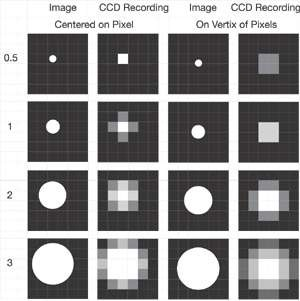
\includegraphics[width=0.4\textwidth]{figures/Orbiter/pixel_size_compare.jpg}
\caption{The pixel size should be selected according to the projected image, \cite{andor2016}.}
\label{fig:pix_size_compare}
\end{figure}
If the object is slightly larger, it will still only be reproduced as a single pixel, with four slightly dim pixels surrounding it. However, when the image covers more than three pixels, the circular object is clearly reproduced. The goal is to sample the object with two to four pixels. This will give the best balance between sensitivity and resolution\cite{sbig2014}. Naturally, the actual object size will depend on the telescope focal length. Matching the sensor pixel size and the focal length will therefore be essential to get high enough sensitivity, without sacrificing resolution.
\item[Speed] The readout speed and therefore the maximal framerate is important to consider, when selecting sensors. Estimated data rates will be calculated to ensure the final design will be realistic.
%\todo[inline]{readout speed, as required by the calculations}
%\item[Dark Current]
%\todo[inline]{dark current (ifikratis)}
%\item[Rad-hard]
%\todo[inline]{sensor rad hard (ifikratis)}
\end{description}
%\todo[inline]{Actual sensor selection missing}
%\subsection{Spacecraft Pointing and alignment}
%\todo[inline]{Akis: Spacecraft Pointing and alignment }
%\todo[inline]{Tip tilt mirror - top down imaging vs. rotating - coverage?}
%\todo[inline]{Which types of camera "movement" will be used to get larger coverage? Tip Tilt? etc.}
\subsection{Imaging Spectroscopy}\label{sec:imaging_spectroscopy}
By combining conventional imaging with spectroscopy, it is possible to obtain both the spatial and spectral information of the lunar surface. This combination is commonly known as imaging spectroscopy. This is illustrated in figure \ref{fig:spectral_information}. In this illustration, the spectral bands has been separated using the white lines. Hyperspectral imaging uses many, relatively narrow bands. In comparison, multispectral imaging uses fewer, broader bands, resulting in a lower spectral resolution. 
\begin{figure}[htb!]
\centering
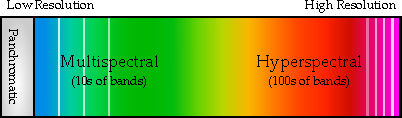
\includegraphics[width=0.75\textwidth]{figures/Orbiter/spectral_information}
\caption{The resolution is defined by the number of bands but also by their bandwidth.}
\label{fig:spectral_information}
\end{figure}
The usefulness of the spectroscopic data depends on the spectral resolution\cite{elowitz2016}. Multispectral imaging makes it possible to detect the presence of simple classes such as vegetation, water and so on. It provides limited information about the actual surface materials. On the other hand, hyperspectral imaging makes it possible to identify surface features, based on the unique spectral signature and thus determine the surface materials, as long as the spectral signature matches an already known substance from the databases. In some cases, it may also be possible to determine subtypes of the materials, such as dirty or clean ice, snow etc\cite{naegeli2015a}. Some materials, such as icy surfaces will have their \textit{spectral fingerprint} within the visible light domain whereas other materials must be observed in the near IR or IR domain to be accurately identified.

Common RGB (color) cameras detects radiation in three bands, typically blue (400 - 470 nm), green (480 - 550 nm) and red (570 - 700 nm) whereas multi- or hyperspectral cameras can acquire images at many more bands, either by adding a spectral dispersion element or filter to the camera\cite{crisp2001}. 
\subsubsection*{Multispectral Imaging}
This type only uses a few extra bands, in addition to the basic color bands (RGB). Around ten bands are commonly used for this imaging technique\cite{elowitz2016}.

One way to implement a simple multispectral camera is to use a filter wheel in front of the detector, illustrated in figure (\ref{fig:filtwheel_miri}). As the selected filter covers the whole detector, the complete image will be filtered and captured. Different filters can be applied in a sequence, effectively creating multispectral data of the lunar surface. 
\begin{figure}[htb!]
\centering
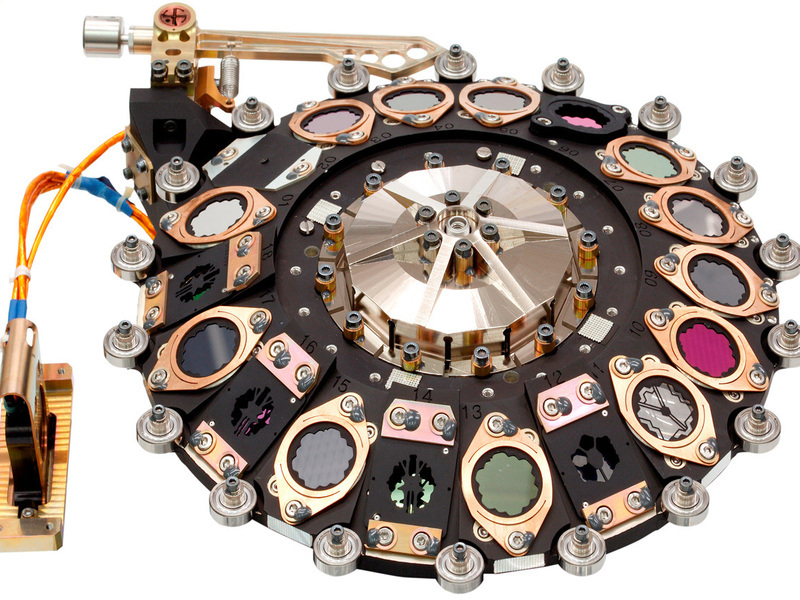
\includegraphics[width=0.30\textwidth]{figures/Orbiter/miri_filterwheel.jpg}
\caption{The filter wheel used for the MIRI instrument onboard the James Webb Space Telescope. Source: MPIA}
\label{fig:filtwheel_miri}
\end{figure}
%\todo[inline]{is it relevant to include this image?}
As the spectral data will be arranged in full frames, only simple post-processing is required to group the spectral "sheets" together, before they are transmitted. However, the filter wheel introduces moving parts, adding to the total weight and complexity of the system. The number of spectral bands will be limited, due to the available space on the wheel. More than 20 bands are not common using this method. Due to the limited number of bands, multispectral imaging will not generate a continuous spectrum but instead generates discrete spectral bands. As the spectral resolution is limited, the usability of the spectral data will be limited as well.

It is important to keep in mind that this method will require additional time when switching between each filter. Due to this delay, each frame may be slightly misaligned, due to the spacecraft movement between frames.
\subsubsection*{Hyperspectral Imaging}
Most imaging spectrometers rely on complex optical systems to split the light into continuous, narrow bands. This includes the Fourier spectrometer and the grating spectrometer. The wedge spectrometer has been proposed in \cite{puschell1999a} as a simpler alternative. By comparing the different spectrometer assemblies in figure (\ref{fig:spec_compare}), the simplicity of the wedge spectrometer is obvious. Due to the limited time available in this course, the Fourier Transform spectrometer has not been analysed further.

\begin{figure}[htb!]
    \centering
    \captionsetup[subfigure]{width=0.25\textwidth}
    \subfloat[Fourier Transform]{
        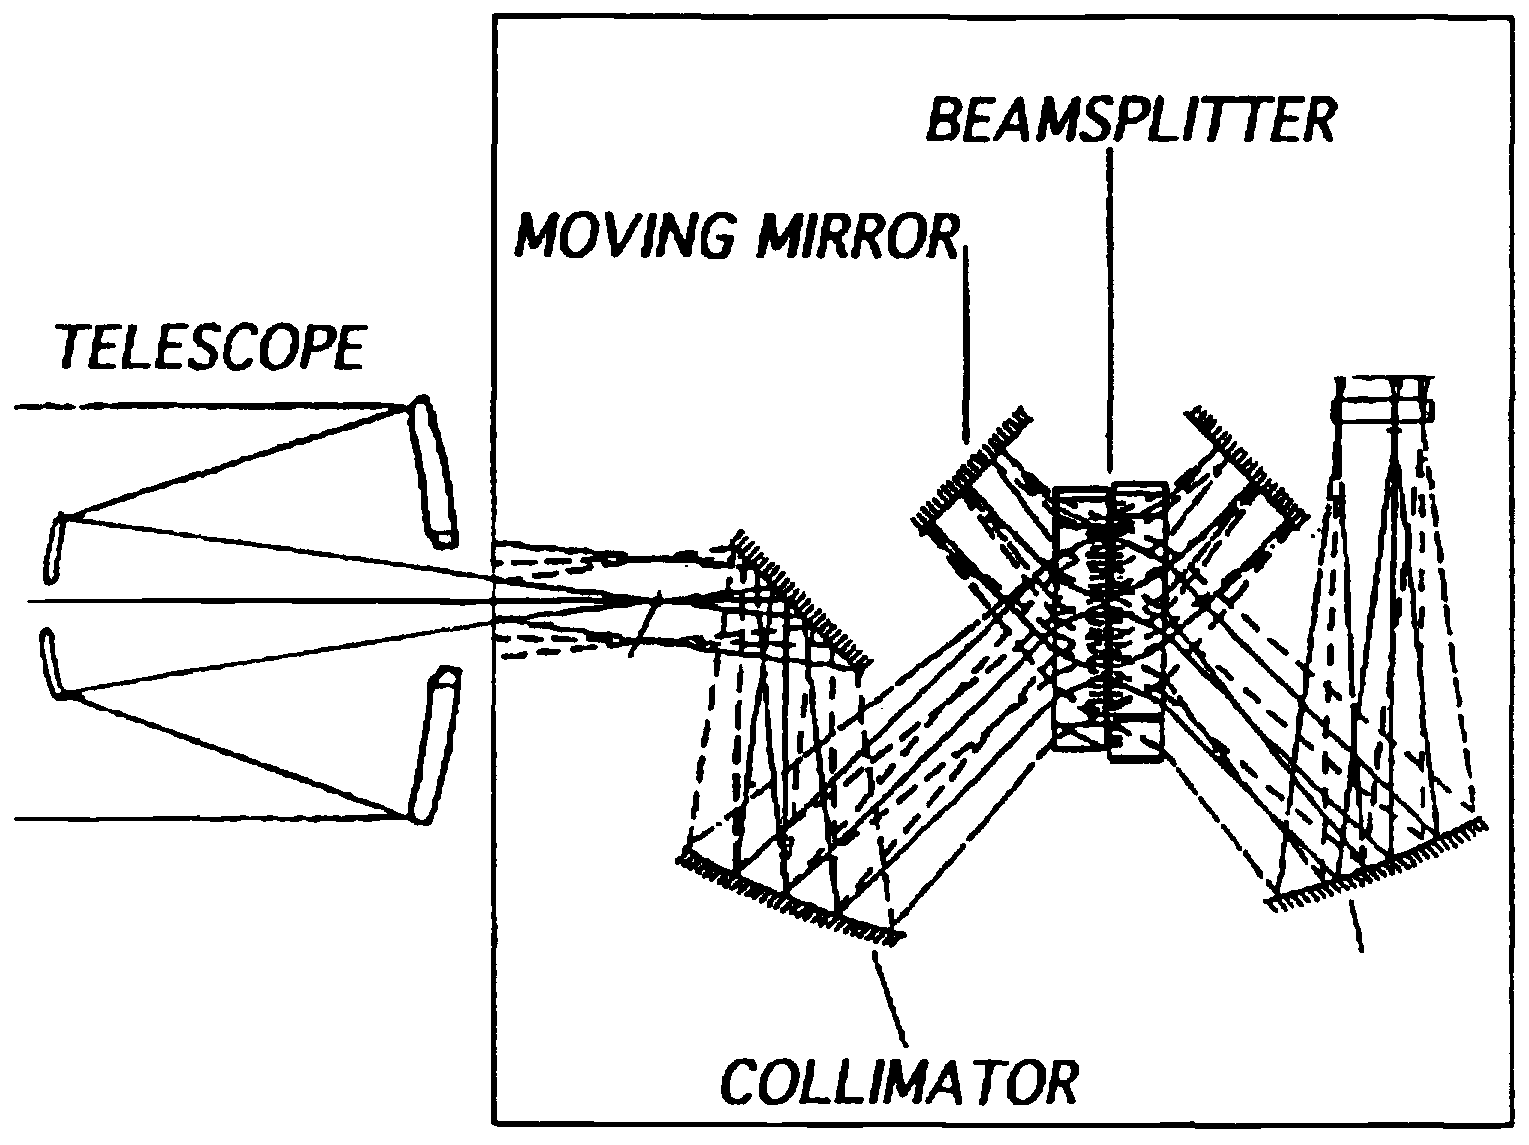
\includegraphics[width=.3\textwidth]{figures/Orbiter/spectrometer_fourier.png}
        \label{fig:spec_fourer}
    }
    \subfloat[Grating]{
        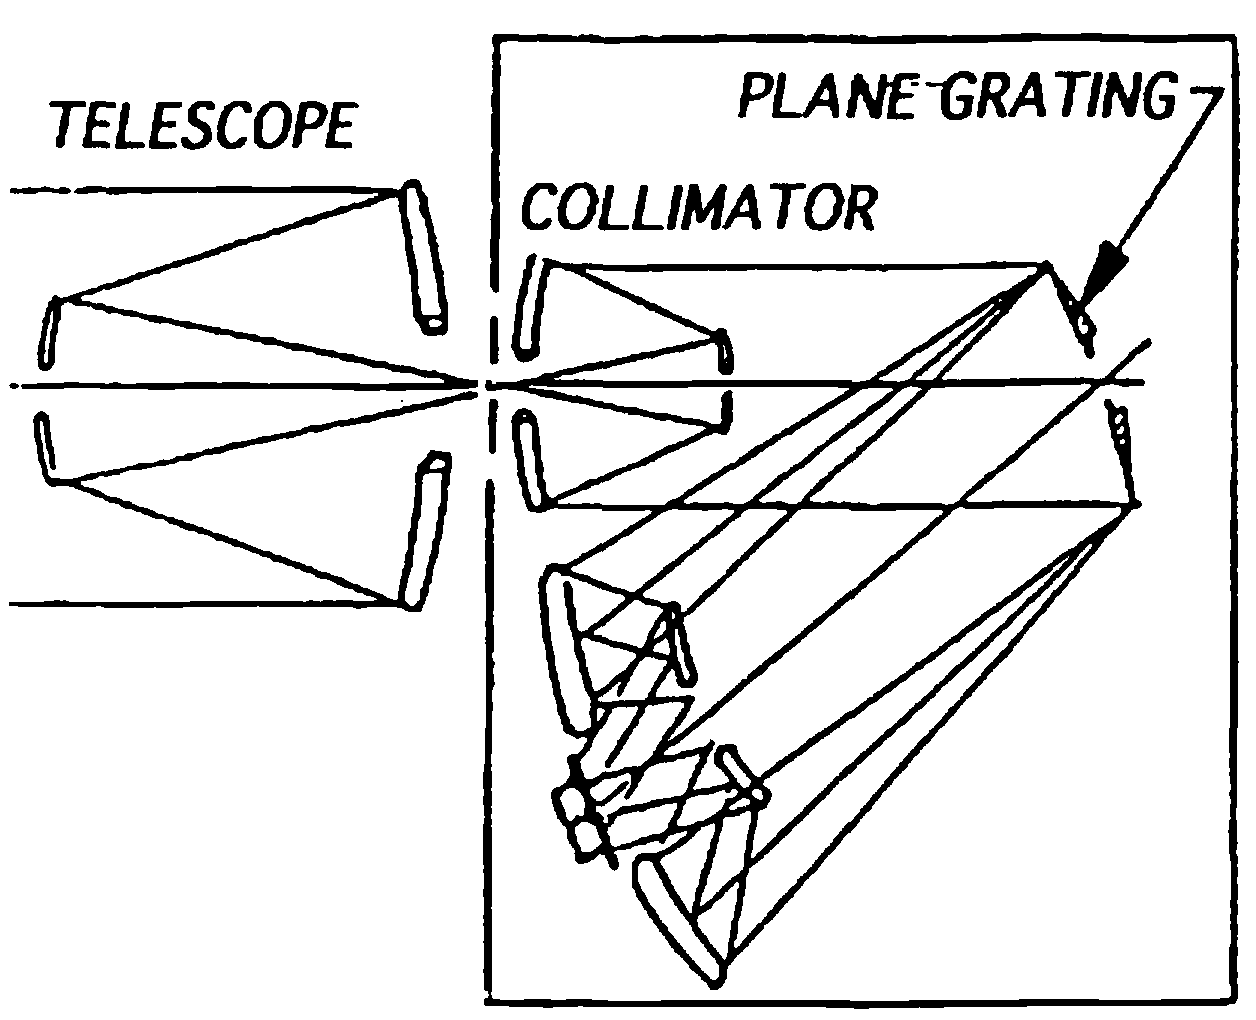
\includegraphics[width=.3\textwidth]{figures/Orbiter/spectrometer_grating.png}
        \label{fig:spec_grating}
    }
    \subfloat[Wedge]{
        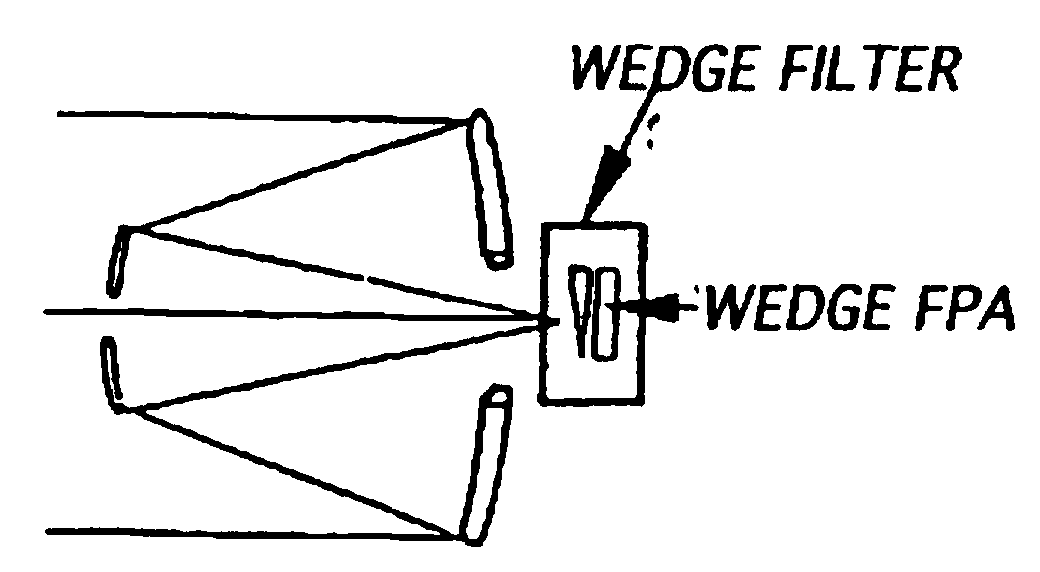
\includegraphics[width=.3\textwidth]{figures/Orbiter/spectrometer_wedge.png}
        \label{fig:spec_wedge}
    }
    \caption{A comparison between spectrometer types. Source:\cite{puschell1999a}.}\label{fig:spec_compare}
\end{figure}

\noindent
The Wedge Imaging Spectrometer could be a suitable candidate for the system, as it will certainly require much less mass than the alternatives while providing better spectral resolution, compared to the simple filter wheel approach. Filter based spectrometers, such as the wedge type (\ref{fig:spec_wedge_acq}) uses a linear variable filter (LVF), where the spectral properties vary linearly on the wedge\cite{joseph2015building}. The filter is constructed by overlaying layers of dielectric film with high and low refractive indexes in a specific pattern. Because of the tapered dielectric coatings of the film, the passband center wavelength for the thin-film stack will essentially depend on the thickness of the stack. Therefore, the center wavelength of the radiation passing through the wedge filter will vary linearly along the tapered edge of the wedge filter\cite{joseph2015building}. This concept is illustrated in figure (\ref{fig:spec_wedge2}).

\begin{figure}[htb]
\centering
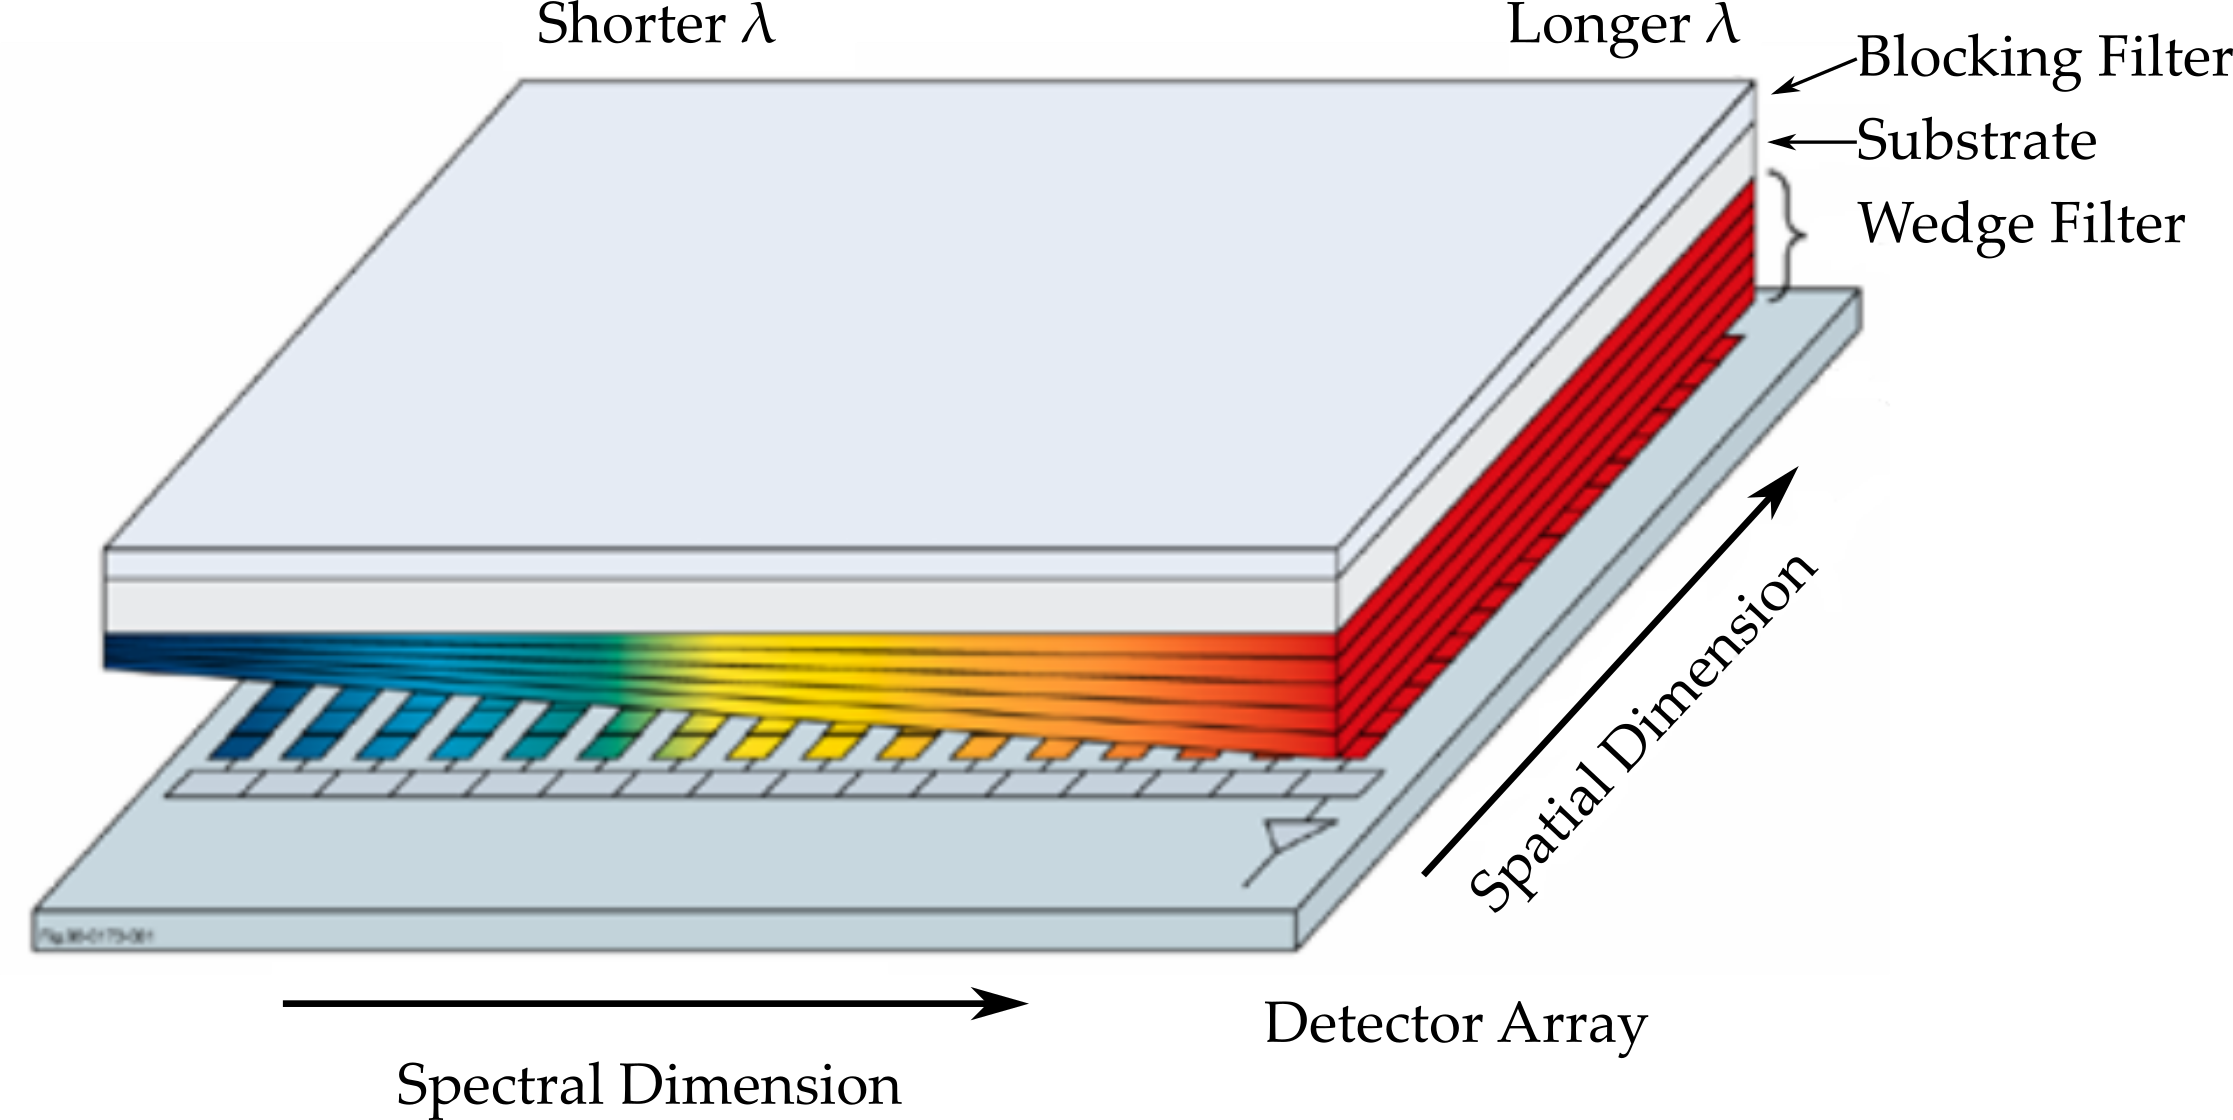
\includegraphics[width=0.65\textwidth]{figures/Orbiter/spectrometer_wedge_3}
\caption{The Linear Wedge Filter, mounted on the detector. Adapted from:\cite{puschell1999a}.}
\label{fig:spec_wedge2}
\end{figure}

\noindent
From the figure, it can be seen how the wedge filter is coupled very close to a 2D detector array, with the coated surface facing the array. A blocking filter, covering the spectral region of interest is mounted on the opposite side of the substrate, to remove out-of-band radiation. Each detector row in the spatial dimension is aligned with a given spectral band, using an even spacing between each band. Therefore, the rows will receive light at different wavelengths.

The filter wheel requires several moving parts and a therefore a larger mass. However, it offers an increased amount of flexibility as the system can easily operate with or without filters applied to the imaging sensor. This makes the method very suitable for the secondary objectives, where a filter is not strictly necessary.

The Grating Spectrometer offers a much higher spectral resolution but is unsuited due to the complex design. It is also not very flexible, as it will not be possible to operate the system without generating spectral data, making it unsuited for the secondary objectives. Due to the limited image acquisition methods possible, it will also not be able to give adequate coverage. The different imaging spectrometers has been compared in table \ref{tab:score_imaging_spectrometer}. 

\begin{table}[htb!]
  \centering
\begin{tabular}{l|l|rrr}
\multicolumn{2}{c|}{\textit{\textbf{Imaging Spectroscopy}}} & \textit{Filter Wheel} & \textit{Grating} & \textit{Wedge} \bigstrut[b]\\
\hline
\textbf{Design Drivers:} & \textit{Simplicity} & 3     & 2     & 5 \bigstrut[t]\\
      & \textit{Flexibility} & 4     & 2     & 3 \\
      & \textit{Physical Req.} & 2     & 2     & 5 \\
      & \textit{Support System Req.} & 3     & 2     & 2 \\
      & \textit{Processing Req.} & 5     & 3     & 3 \\
      & \textit{Redundancy} & 2     & 1     & 4 \bigstrut[b]\\
\hline
\textbf{Primary:} & \textit{Spectral Resolution} & 1     & 5     & 5 \bigstrut[t]\\
\textbf{} & \textit{Coverage} & 3     & 2     & 4 \bigstrut[b]\\
\hline
\textbf{Secondary} & \textit{Orbit Determination} & 4     & 1     & 3 \bigstrut[t]\\
      & \textit{Geo-location} & 4     & 1     & 3 \\
      & \textit{Topography} & 4     & 1     & 3 \bigstrut[b]\\
\hline
\multicolumn{1}{r}{\textbf{Total:}} & \textit{} & 35/55 & 22/55 & 40/55 \bigstrut[t]\\
\end{tabular}%
  \caption{The score table for the Imaging Spectrometer. 5 is the highest grade given.}
  \label{tab:score_imaging_spectrometer}%
\end{table}%

The wedge spectrometer scores slightly better than the filter wheel method. The system trades higher processing requirements and higher support system requirements with a very simple and relatively flexible system. Processing power is relatively cheap on the spacecraft but the higher requirements from the support systems, such as the attitude control, will be the main challenge with this design. However, this is to be expected, when performing surface imaging.

A high spectral resolution and good coverage is possible with the wedge spectrometer but it can be seen how the system performs slightly worse at the secondary objectives. This is caused by the limitations of the wedge filter, as it can only capture an image frame by scanning, operating as a push broom imager. The push broom technique is not very suitable for capturing opnav images or topographic images.

To improve the performance, a simple solution is suggested. By having an extra detector, the wedge filter and sensor assembly can be removed from the telescope and switched with a bare detector. If a 2D detector is used, this makes it possible to capture full frame images with no filter applied. While it will require moving parts, it will greatly improve the performance of the non-spectral imaging capabilities of the system.
\subsubsection*{Image Acquisition}
When considering what spectrometer to use for the imaging system, it is not just a  matter of selecting the lightest and simplest design. Examining the assembly of the two different spectrometer systems makes it clear how the images will be acquired and how the output data will be ordered. The image acquisition method is important to consider, as the ordering of the generated data can affect the post-processing system significantly. Common methods include whisk-broom/push-broom (pixel or line) or staring (frame) captures. The two spectrometer assemblies are shown in figure (\ref{fig:spec_acquisition_compare}). 

\begin{figure}[htb!]
    \centering
    \captionsetup[subfigure]{width=0.45\textwidth}
    \subfloat[Dispersive Type]{
        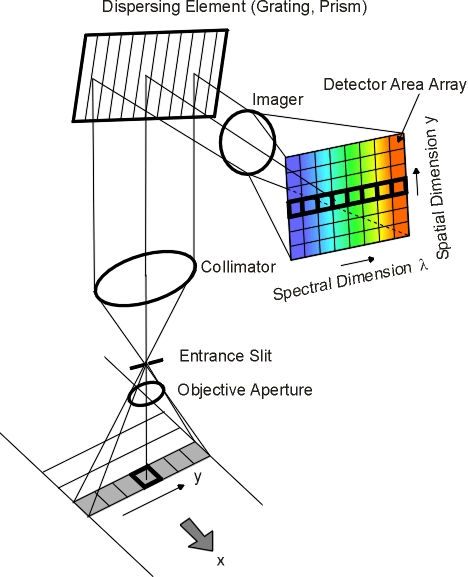
\includegraphics[width=.48\textwidth]{figures/Orbiter/spectrometer_colli_nieke.jpg}
        \label{fig:spec_dispersion_acq}
    }
    \subfloat[Wedge Filter Type]{
        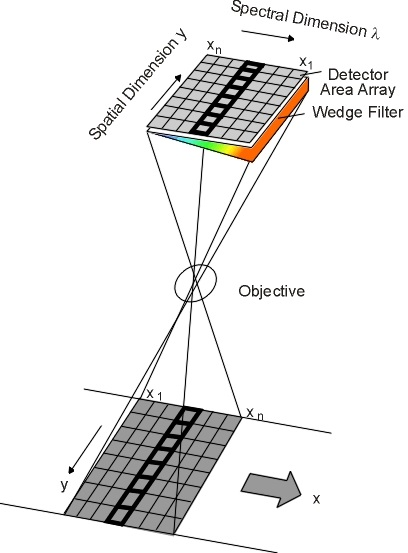
\includegraphics[width=.48\textwidth]{figures/Orbiter/spectrometer_wedge_nieke}
        \label{fig:spec_wedge_acq}
    }
    \caption{A comparison between acquisition methods. Adapted from:\cite{nieke1997a}.}\label{fig:spec_acquisition_compare}
\end{figure}

The first method (\ref{fig:spec_dispersion_acq}) uses gratings or prisms as the dispersion element. The element separates the incoming electromagnetic radiation into different wavelengths. A single ground pixel is dispersed and focused onto different locations on the array detector\cite{nieke1997a}, resulting in a whisk-broom acquisition but with each "whisk" covering a specific spectral band.

The wedge spectrometer is realised by mounting the detector filter assembly in the focal plane of the imaging optics (\ref{fig:spec_wedge_acq}), \cite{joseph2015building} and \cite{nieke1997a}. By placing the wedge filter along the direction of movement, the imaging system is able able to capture a frame of each cross strip from $x_1$ to $x_n$. With With $n$ strips covering different surface areas, each cross strip will correspond to a specific spectral band, depending on the region on the wedge filter. If a 1D array detector is used (i.e a detector that is 1 pixel wide), the spectrometer will be acquiring each spectral band in a whisk-broom fashion. By using a 2D array detector instead, the spectrometer will acquire the spectral bands in a push-broom fashion. Each recorded frame will contain $n$ different ground strips corresponding to each of the spectral bands in the filter. When the spacecraft moves, each ground strip will be imaged by different positions on the wedge filter, thus creating multispectral data for each surface area.

Unlike the dispersive type, where the full spectra of a single pixel is recorded in a single frame, the wedge filter requires reorganising the data, before the hyperspectral cube can be generated for a given surface area. With $n$ spectral bands, the first and the last band for a given ground strip will be collected with a time difference of $(n-1)\cdot \tau$. As the spectral bands for each ground strip will not be linked, the the attitude stability of the spacecraft will therefore play a major role in the band-to-band registration accuracy\cite{joseph2015building}, therefore requiring more from the support systems. The wedge filter imaging sequence is illustrated in figure (\ref{fig:wedge_filt_img_sequence}), where the surface area is illustrated by the blue square.

\begin{figure}[htb!]
\centering
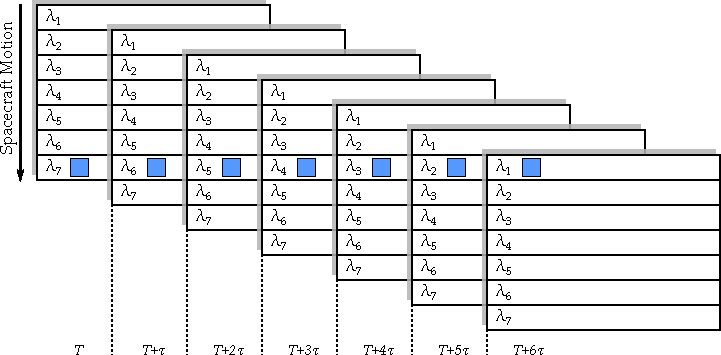
\includegraphics[width=\textwidth]{figures/Orbiter/wedge_filt_img_sequence.pdf}
\caption{The wedge filter imaging sequence. Adapted from:\cite{joseph2015building}.}
\label{fig:wedge_filt_img_sequence}
\end{figure}

\noindent
At time $T$, the ground area will be viewed by channel $\lambda_7$, at $T+\tau$ the area is viewed by channel $\lambda_6$ and so on. Therefore, it is necessary to use post-processing to link the spectral data together. As the raw data cannot be transmitted due to communication constraints, they must be processed and reordered on the spacecraft. A large part of the image system is therefore to design an efficient and fast processing system that can process and store the images faster than they are generated.

When operating the spectrometer as a push-broom imager, a large amount of data will be generated. Additionally, the dispersion spectrometer and the wedge spectrometer generates data in a different order, when compared to the simpler filter wheel method, apparent from figure (\ref{fig:wedge_filt_img_sequence}). Each section of the imaging sensor is dedicated to a specific spectral band. 

Unlike the full frame capture used by the filter wheel, the push-broom techniques generate all spectral data in parallel. With many parallel data streams, it is a problem very suitable for a parallel processing system, where each spectral data stream is computed individually.
%\todo[inline]{other aspects to consider when designing hyperspectral cameras (see joseph2015building, page 272)}
\section{Imaging System Proposal}
The imaging system consists of several subsystems. Based on the previous analysis of each subsystem, the overall imaging system will now be specified.
\subsection{Imaging System Structure}
A dual camera system structure, using both a NAC and a WAC is proposed for the final design. The selected system structure requires a more complicated design but will make it possible to perform both the primary and secondary objectives at a high performance. As the surface imaging is not the primary mission objective, it is important that the system can provide useful data for the remaining groups.

The two cameras will be very suited for capturing both low and high resolution imaging at the same time. Some of the secondary objectives are better suited with the WAC (lander tracking and opnav imaging) whereas both cameras will be suited for the geolocation operation. The two cameras can substitute each other to a degree, providing built in redundancy. Therefore, the mission can still continue, if one camera fails. However, as the WAC is complicated to replace, it is suggested that a secondary WAC is included as a backup. Operating the primary and secondary WAC together will also make it possible to increase the surface coverage and make it possible to generate stereographic images. 
%\todo[inline]{diagram of the imaging system structure}
%\subsection{Telescope and Detectors}
%\todo[inline]{Which design has been selected for Telescope and Detectors and why?}
%\subsection{Spacecraft Pointing and alignment}
%\todo[inline]{Selecting the Final pointing method and argument for this selection}
\subsection{Imaging Spectroscopy and Acquisition}
Combining the suitable parts from both the filter wheel and the wedge spectrometer results in the proposed solution for this subsystem. The wedge filter provides the spectral data but can be removed from the sensor, making it possible to capture the full frame images suited for the secondary objectives. In this way, high performance is ensured for both the imaging and spectroscopy mode. 

The system design remains simple, but requires slightly more moving parts for switching the filter. However, it is the increased support system requirements (attitude control, processing and storage resources) that will drive the cost. Naturally, surface mapping using a high spectral resolution will require more from the support system and cannot be avoided. However, if the support systems are already required and will be shared, this will not be an issue.

Image acquisition can be done in two different ways, when using the wedge spectrometer - using whisk-broom or push-broom. The main difference is the coverage or swath\footnote{Swath; the width of the lines sweeping over the surface} per flyby. Naturally, a large coverage is required to minimise the number of flybys required, making push-broom a suitable image acquisition method. This approach will require a 2D array detector, as each spectral channel has a matching area on the detector. The detector will capture a full frame at a time but the spectral data will be structured in individual areas on the detector. As the data are structured in this fashion, it is necessary to process and store the images, before they can be transmitted to the ground station.
%\subsection{System Flaws}
%\todo[inline]{System flaws? Is this the best solution?}
%\subsection{Similar Systems}
%\todo[inline]{Currently Available NAC/WAC - See powerpoint (Ifikratis)}
%\todo[inline]{What changes will be necessary to adapt the current systems?}
%\newpage
\section{Support Systems Overview}
%\todo[inline]{Is the support system section complete?}
The imaging system requires several support systems that will either be provided as part of the imaging system or shared between the other systems on the orbiter. A comparison of the cost drivers for the different support systems are shown in table \ref{tab:design_cost_driver}. Only a few of the support systems are not shared with other on-board instruments.
\begin{table}[htb!]
  \centering
\begin{tabular}{p{4cm}|p{11cm}}
\toprule
      & \textbf{Design and cost drivers} \\
\midrule
\textit{Orbit Determination and Attitude Control} & Essential for navigation, accuracy required by imaging system \\
\textit{Image Processing} & Essential for imaging system \\
\textit{Generic Processing} & Generic processing power is essential for the orbiter. \\
\textit{Data Storage} & A large data storage is necessary for the imaging system but other systems will also require data storage. \\
\textit{Thermal Control} & Thermal control is crucial for the orbiter, especially due to the RTG. Thermal control is also essential for the imaging system. \\
\textit{Power System} & A power system must be present for both the imaging system and remaining systems. \\
\textit{Radiation Protection} & Radiation protection is essential for all electronics, including communication. Especially the detector (CCD) will require protection. \\
\bottomrule
\end{tabular}%
  \caption{Comparison of the design and cost drivers used by the orbiter.}
  \label{tab:design_cost_driver}%
\end{table}%
\subsection{Attitude Determination and Control}
To ensure the stability and achieve the correct orientation of the orbiter, a complete attitude determination and control system will be needed. The four gravity assist flybys, along with the planned close encounters with Europa, needed for surface imaging, increase the requirements for high accuracy and reliability of the attitude subsystem.

The closest approach to Europa is at a distance of 100 km, using an average flyby speed of 3.3 km/s and an angular velocity of approximately 0,002rad/s (or 0,1146$^{\circ}$/s). This defines the steering and pointing accuracy requirements of the orbiter. 
\begin{table}[htb!]
  \centering
    \begin{tabular}{|p{4,7 cm}|p{4,7 cm}|p{4,7 cm}|}
    \hline
    \textbf{Stearing} & \textbf{Effect on Spacecraft} & \textbf{Effect on ADC Selection} \bigstrut\\
    \hline
    Nominal rates 0,05 - 0,5 deg/sec & Minimal & Thrusters \bigstrut\\
\cline{3-3}          &       & Reaction wheels \bigstrut\\
    \hline
    \end{tabular}%
    \caption{Stearing requirements \cite {spacemissionanalysis}}
  \label{tab:stearing_req}%
\end{table}%

\begin{table}[htb!]
  \centering
    \begin{tabular}{|p{4,7 cm}|p{4,7 cm}|p{4,7 cm}|}
    \hline
    \multicolumn{1}{|c|}{\textbf{Required Accuracy}} & \multicolumn{1}{c|}{\textbf{Effect on Spacecraft}} & \textbf{Effect on ADC Selection} \bigstrut\\
    \hline
          &       & Need for accurate attitude reference (Star Tracker $\mu$ASC) \bigstrut\\
\cline{3-3}    0,1 - 1 deg & 3-axis and momentum - bias stabilisation & Reaction wheels \bigstrut\\
\cline{3-3}          &       & Thrusters for momentum unloading and coarse control \bigstrut\\
    \hline
    \end{tabular}%
    \caption{Pointing accuracy requirements \cite {spacemissionanalysis}}
  \label{tab:point_acc_req}%
\end{table}%
For the proposed attitude determination system, a set of four micro-Advanced Stellar Compass ($\mu$ASC) star trackers (Table \ref{tab:masc}), while electrically-powered reaction wheels will be responsible for the 3-axis control. External disturbance torques will saturate eventually the wheel speed of the reaction wheels, so a set of gimballed thrusters are necessary for momentum unloading ensuring attitude stabilisation.

\begin{table}[htb!]
  \centering
    \begin{tabular}{|r|c|}
    \hline
    Initial acquisition & 30mS \bigstrut\\
    \hline
    \multicolumn{1}{|c|}{Accuracy} & 1” \bigstrut\\
    \hline
    \multicolumn{1}{|c|}{Attitude rate} & Up to 10$^{\circ}$ /sec \bigstrut\\
    \hline
    \multicolumn{1}{|c|}{Update rate} & Up to 20Hz \bigstrut\\
    \hline
    \multicolumn{1}{|c|}{Availability} & 99,995\% \bigstrut\\
    \hline
    \multicolumn{1}{|c|}{Power} & 1.9W \bigstrut\\
    \hline
    \multicolumn{1}{|c|}{Mass} & 425g \bigstrut\\
    \hline
    \multicolumn{1}{|c|}{Size} & DPU: 10x10x4.5cm CHU: 5x5x5cm \bigstrut\\
    \hline
    \multicolumn{1}{|c|}{Lifetime} & $>$30 years \bigstrut\\
    \hline
    \multicolumn{1}{|c|}{Reliability} & 99,999\% \bigstrut\\
    \hline
    \end{tabular}%
    \caption{$\mu$ASC star tracker specifications \cite {masc}}
  \label{tab:masc}%
\end{table}%
Selection of the proposed combination assures an autonomous and high accuracy pointing of the imaging system and the pointing of the high gain antenna toward Earth as well. 
%\subsubsection*{Imaging System}
This subsystem is required to make it possible to follow a specific pattern, increasing the surface coverage. The accuracy of the attitude control is partially driven by the specific accuracy requirements by the imaging system. However, attitude control is a crucial part of the navigation and orbit determination. Attitude control is also required to maintain a stable communication link to the ground station. 

As previously suggested, the imaging system could be used to generate the opnav images used for orbit determination. Using the imaging system for both mapping and for tracking could be possible, but it may be difficult to do it at the same time. It may also require a different camera design, as both the relatively bright lunar surface and the dark star background must be possible to photograph.

If the imaging system cannot be used for both tasks, a separate orbit (and orientation) determination subsystem is required in addition to the imaging system. Naturally, actuators for correcting the trajectory will also be required for the attitude control. These support systems will be needed - with or without an imaging system, as they are an essential part of any spacecraft navigation system. Therefore, it is not expected that the imaging system will be driving the design requirements alone.
\subsection{On-board Processing and Data Management}
The imaging system requires a processing system to prepare the images, before they are transmitted. The system will filter and compress the data from the imaging system, only sending the instructed data down to the ground station. The communication window will be very short, limiting the amount of data that can be transmitted. Therefore, on-board storage is required. As the digital image processing system will most likely be a problem specific (ASIC or FPGA) implementation, it will only be useful for the imaging system and other specific problems such as data compression. On the other hand, the storage bank(s) can certainly be shared between the rest of the systems requiring a storage buffer between communication windows, as long as these systems do not require a huge data storage. Any other programmable processors required by the imaging system can also be shared with the other instruments on the orbiter.
\subsection{Thermal Management}
Thermal control of the spacecraft is essential, as it is required to ensure the electrical and mechanical parts of the imaging system will be operating within a specific temperature range\cite{fortescue2011a}. Often, the electrical and mechanical systems will only operate efficiently and reliably, if they are kept within this range. Often, the parts must be operated around room temperature. Most spacecraft originated as parts meant for terrestrial use and were therefore developed under this environment.

Most electronic systems, such as the microprocessors and power supply circuits should be operating in a temperature range of $-15^\circ$C to $+50^\circ$C. Mechanical mechanisms such as momentum wheels, gyroscopes and telescope shutters must be operated between $0^\circ$C to $+50^\circ$C and batteries between $0^\circ$C to $+20^\circ$C\cite{fortescue2011a}.

Thermal control is already required by the electrical communication hardware so the imaging system is not the only design and cost driver here. An advanced thermal system is also required to move the heat from the RTG away from the spacecraft, keeping the spacecraft from overheating. At the same time, a temperature difference across the peltier elements must be maintained, to generate power. 

However, the imaging system will require a very high structural stability to maintain high pointing accuracy. This means the thermally induced distortion must be minimised or controlled as part of the orbiter design. The CCD detector used in the cameras will also benefit greatly from a lower temperature. The thermal energy is enough to excite electrons into the image pixels, indistinguishable from actual photo-electrons. This event generates noise and is also known as \textit{dark current}. Fortunately, the dark current can be decreased if the CCD temperature is reduced. Typically, the dark current rate can be reduced by 50\%, if the CCD temperature is reduced by $6-7^\circ$C \cite{sbig2014}. For the KAF-8300 CCD mentioned in this source, the noise has almost disappeared, when the CCD is cooled to $-30^\circ$C. It is expected that a temperature between $-30^\circ$C to $-50^\circ$C would be a suitable choice but it depends on the specific CCD.
%\todo[inline]{Specific CCD requirements}
%\todo[inline]{Thermal system diagram?}
\subsection{Power Systems}
Power system design utilises a single General Purpose Heat Source - Radioisotope Thermoelectric Generator (GPHS-RTG) Fig.\ref{fig:rtg}. The deep space nature and the multi-year duration of this mission, renders the use of an RTG necessary. At a 5.2 AU distance from the sun, selection of a solar PV-battery configuration is considered prohibited, taking into account the weak solar flux and the limited the mass budget. Furthermore, excess thermal power produced by the RTG can be exploited for the heating needs of the internal electronic components.

%\subsubsection*{General Purpose Heat Source - RTG} 
Utilizing the natural decay of plutonium-238 oxide (with 83.9\% , GPHS-RTG is capable of delivering a power output of 290 watts of electrical power at BOL. With a long half-life of 87.7 years, fuel is able to provide up to 40,000 operational life-hours making it the ideal choice for our long duration mission. However a 0.8\% annual decrease of thermal power output is expected, reaching 250 watts at EOL. $PuO_2$ is encapsulated into 18 modules with the form of pellets, with each module providing 245 watts of thermal power, with a total output of 4,410 watts. Each pellet is contained within a welded iridium alloy for safety reasons, to avoid oxidation in case of an impact. 

A thermionic converter made of 572 silicon-germanium thermoelectric elements uses the thermal power produced from the decaying material, converting it to electrical power. Nominal hot shoe temperature is about 1270 K and the converter can reach efficiencies up to 7\%. The whole GPHS-RTG module has a diameter of 0.422 m and length of 1.13 m and weights approximately 56 kg. Total amount of fuel required, stands at 10.9 kg of $PuO_2$ with 9.71 kg being plutonium-238.

\begin{figure}[htb]
\centering
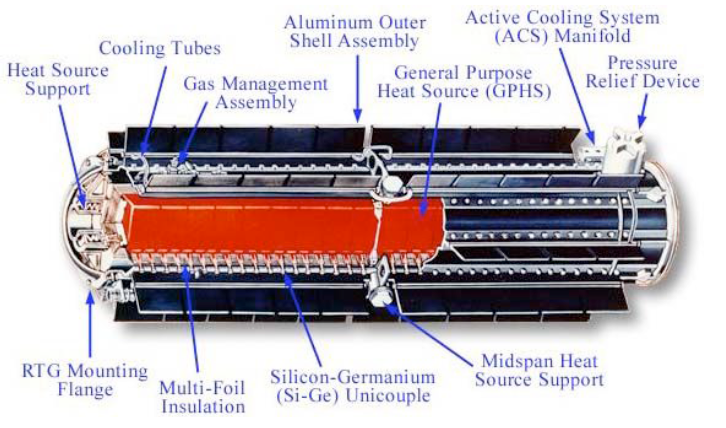
\includegraphics[scale=0.6]{figures/Orbiter/rtg.png}
\caption{GPHS-RTG cutaway. \cite{rtg}}
\label{fig:rtg}
\end{figure}

\noindent
The power system design of the orbiter integrates the second RTG module on board the lander, in order to compensate any power needs higher than the available output of the orbiters power source. The imaging system will not be the primary design driver for this part, as the power system will be required - with or without an imaging system. It is also important to consider that the imaging system will mainly be operating, when the penetrator and lander is still docked on the orbiter. At this point, the penetrator and its instruments will not be operating.
\subsection{Radiation Shielding}
The radiation environment of Jupiter can be very demanding for any mission in respect to the necessary protection needed against highly energetic particles. Protons and other heavy ions fluxes appear similar to other interplanetary missions. On the other hand, high electron fluxes should be considered the main danger of this mission.
Below in fig. \ref{fig:eleprotflux}, the expected electron and proton fluxes are presented for one year duration trajectory. Estimated flux was calculated based on the final orbit selection of the orbiter.

\begin{figure}[htb!]
\captionsetup[subfigure]{width=0.45\textwidth}
\subfloat[Electrons]{
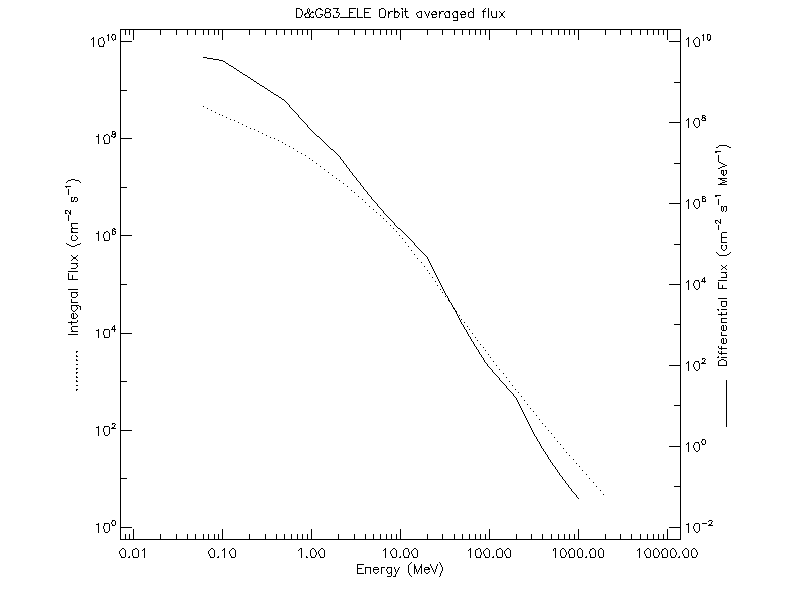
\includegraphics[width=0.48\linewidth, height=5cm]{figures/Orbiter/electrons.png}
\label{fig:elec}
}
\subfloat[Protons]{
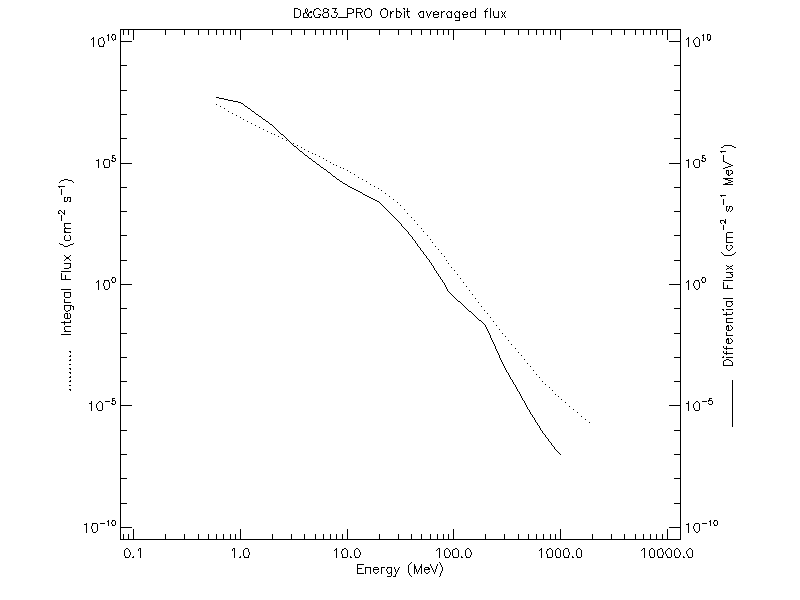
\includegraphics[width=0.48\linewidth, height=5cm]{figures/Orbiter/protons.png}
\label{fig:prot}
}
 
\caption{Average spectra of trapped electrons and protons, SPENVIS}
\label{fig:eleprotflux}
\end{figure}
Results are summarized on table \ref{tab:particleflux}. 
% Table generated by Excel2LaTeX from sheet 'Sheet1'

\begin{table}[htb]
  \centering
    \begin{tabular}{|c|c|c|}
    \hline
    \textbf{} & \multicolumn{2}{c|}{\textbf{Flux ($cm^2/s$)}} \bigstrut\\
\cline{2-3}    \textbf{Particle Energy (MeV)} & \textbf{Electron} & \textbf{Proton} \bigstrut\\
    \hline
    10    & 9.90E+05 & 4.83E+04 \bigstrut\\
    \hline
    20    & 1.92E+05 & 8.36E+03 \bigstrut\\
    \hline
    30    & 6.74E+04 & 2.07E+03 \bigstrut\\
    \hline
    50    & 1.83E+04 & 1.94E+02 \bigstrut\\
    \hline
    100   & 3.34E+03 & 4.20E+00 \bigstrut\\
    \hline
    \end{tabular}%
    \caption{Trapped particle fluxes for Jupiter, SPENVIS (D G83 PRO)}
    \label{tab:particleflux}
\end{table}%

For an effective shielding against radiation, three levels of protection are advised. Spacecraft structure along with the side mounted fuel tanks will provide the first level collateral protection against the external radiation. However, external shielding can only be limited, due to mass constrains and structural limitations, thus making a second level protection necessary. 

\noindent
A vault-like structure in the heart of the spacecraft,containing all the electronic components, will offer the second level protection. Wall thickness of the vault will be 6-cm thick and be constructed out of aluminum. This configuration will bring the annual TID of the internal electronics to approximately 100 krad, based on the obtained results (table \ref{tab:thicknessalum} and fig. \ref{fig:shield}) for one year of radiation exposure under the selected orbit near Europa. Assuming the use of existing aerospace radiation hardened components rated at 300 krad, orbiter's lifetime will be limited to at least three years on a near Europa orbit. Localized shielding with high-Z materials on individual components , will form the third level of protection. Sensitive electronics, such as Single-Level-Cell Flash Memories, under a TID exceeding 65 krad, present retention errors and block erase fails, thus the use of local protection is vital. 
 
% Table generated by Excel2LaTeX from sheet 'Sheet1'
\begin{table}[htbp]
  \centering
  
    \begin{tabular}{|c|c|c|c|c|c|c|}
    \hline
    \multicolumn{3}{|c|}{\textbf{Aluminum thickness}} &       &       & \textbf{Brems- } &  \bigstrut\\
    \hline
    \textbf{(mm)} & \textbf{(mils)} & \textbf{(g cm2)} & \textbf{Electrons} & \textbf{Protons} & \textbf{strahlung} & \textbf{Total (krad)} \bigstrut\\
    \hline
    0.5   & 19.685 & 0.135 & 1.81E+08 & 2.44E+06 & 6.12E+05 & 184200 \bigstrut\\
    \hline
    1     & 39.37 & 0.27  & 8.20E+07 & 1.03E+06 & 3.57E+05 & 83400 \bigstrut\\
    \hline
    2     & 78.74 & 0.54  & 3.68E+07 & 3.13E+05 & 2.15E+05 & 37350 \bigstrut\\
    \hline
    3     & 118.11 & 0.81  & 2.12E+07 & 1.21E+05 & 1.63E+05 & 21530 \bigstrut\\
    \hline
    4     & 157.48 & 1.08  & 1.37E+07 & 5.74E+04 & 1.35E+05 & 13930 \bigstrut\\
    \hline
    5     & 196.85 & 1.35  & 9.79E+06 & 3.18E+04 & 1.19E+05 & 9936 \bigstrut\\
    \hline
    10    & 393.7 & 2.7   & 3.60E+06 & 3.91E+03 & 9.07E+04 & 3692 \bigstrut\\
    \hline
    15    & 590.55 & 4.05  & 2.00E+06 & 9.66E+02 & 8.25E+04 & 2083 \bigstrut\\
    \hline
    20    & 787.4 & 5.4   & 1.26E+06 & 3.53E+02 & 7.78E+04 & 1339 \bigstrut\\
    \hline
    25    & 984.25 & 6.75  & 8.15E+05 & 1.69E+02 & 7.36E+04 & 888.7 \bigstrut\\
    \hline
    30    & 1181.1 & 8.1   & 5.21E+05 & 1.00E+02 & 6.98E+04 & 591.1 \bigstrut\\
    \hline
    35    & 1377.95 & 9.45  & 3.30E+05 & 6.94E+01 & 6.63E+04 & 395.8 \bigstrut\\
    \hline
    40    & 1574.8 & 10.8  & 2.10E+05 & 5.46E+01 & 6.31E+04 & 272.8 \bigstrut\\
    \hline
    45    & 1771.65 & 12.15 & 1.38E+05 & 4.40E+01 & 6.00E+04 & 198.1 \bigstrut\\
    \hline
    50    & 1968.5 & 13.5  & 9.55E+04 & 3.73E+01 & 5.73E+04 & 152.8 \bigstrut\\
    \hline
    55    & 2165.35 & 14.85 & 6.92E+04 & 3.13E+01 & 5.49E+04 & 124.2 \bigstrut\\
    \hline
    60    & 2362.2 & 16.2  & 5.23E+04 & 2.64E+01 & 5.28E+04 & 105.1 \bigstrut\\
    \hline
    65    & 2559.05 & 17.55 & 4.07E+04 & 2.27E+01 & 5.07E+04 & 91.49 \bigstrut\\
    \hline
    \end{tabular}%
    \caption{TID versus Aluminum shielding thickness for one year of exposure, SPENVIS (SHIELDOSE-2Q)}
  \label{tab:thicknessalum}%
\end{table}%


\begin{figure}[htb!]
\centering
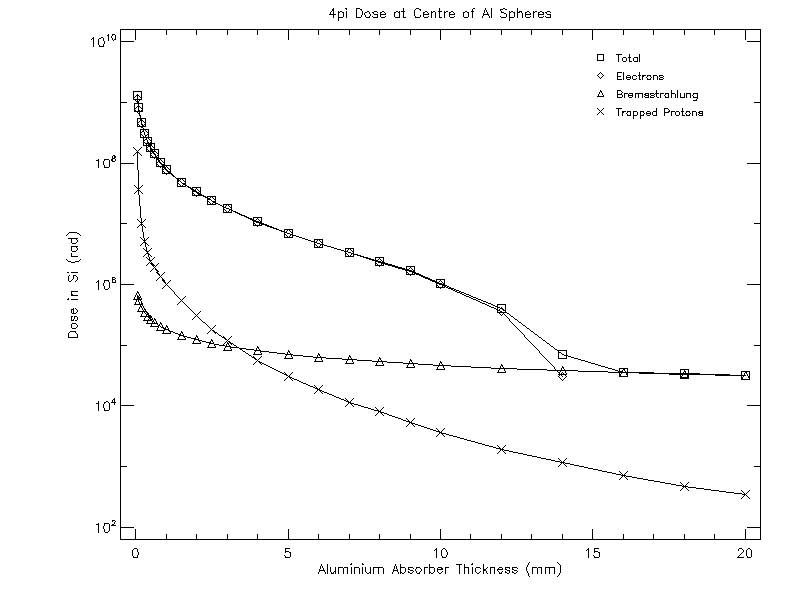
\includegraphics[scale=0.4]{figures/Orbiter/alvsrad.png}
\caption{Radiation levels versus aluminum shielding thickness. SPENVIS (SHIELDOSE)}
\label{fig:shield}
\end{figure}
The CCD of the optical instrument makes the shielding design slightly more complicated. The basic design requires the sensor to be outside of the vault thus subjecting it to higher TID. To compensate that, the sensor will be surrounded with high-Z material (Ta, Ti) shielding, with a retracting gate that will expose the CCD during observational periods and provide protection on non-operational time frames.
%\todo[inline]{radiation protection driven by the sensitive CCD and control circuits.}
%\todo[inline]{dynamic radiation shielding?}
\newpage
\section{Imaging System Design}
\subsection{Telescope and Camera}
When designing the telescope, the required ground resolution and the working range are important parameters to consider. At this point, the ground resolution is known but the orbit parameters has not been completely specified. Therefore, it is assumed that the working range of the imaging system will be between 2000 and 100 km during the flyby while the mpp should be 100 m/pixel for the WAC and 0.5 m/pixel for the NAC, as previously defined.
%\todo[inline]{Refer to ifikratis Cassini image analysis}
The specified ground resolution for the WAC refers to the required resolution at the far distance of the orbit, 2000 km. The ground resolution of the NAC refers to the resolution when at the closest approach, as it is not realistic to maintain a resolution of 0.5 m at 2000 km. 

For the following analysis, the sensor parameters and the required resolution has been specified in table (\ref{tab:ccd_calc_parameters}). These parameters are used for all the remaining calculations and estimates.
%\todo[inline]{refer to CCD selection}
\begin{table}[htb!]
  \centering
\begin{tabular}{l|l|r|r|l}
\textit{\textbf{Calculation Parameters}} & \textit{abbreviation} & \textit{WAC} & \multicolumn{1}{r}{\textit{NAC}} &  \bigstrut[b]\\
\cline{1-4}\textbf{Working Range} & h     & 2000  & 100   & [km] \bigstrut[t]\\
\textbf{Ground Resolution\tablefootnote{The ground resolution per pixel, for the worst case distance}} & mpp   & 100   & 0.5   & [m] \\
\textbf{CCD Resolution H} & $CCD_{res,h}$ & 1024  & 1024  & [pix] \\
\textbf{CCD Pixel Size H} & $CCD_{pix,h}$ & 0.0074 & 0.0074 & [mm] \\
\textbf{CCD Size H} & $CCD_{size,h}$ & 7.5776 & 7.5776 & [mm] \bigstrut[b]\\
\cline{1-4}\textbf{CCD Resolution V} & $CCD_{res,v}$ & 1024  & 1024  & [pix] \bigstrut[t]\\
\textbf{CCD Pixel Size V} & $CCD_{pix,v}$ & 0.0074 & 0.0074 & [mm] \\
\textbf{CCD Size V} & $CCD_{size,v}$ & 7.5776 & 7.5776 & [mm] \\
\end{tabular}%
  \caption{The parameters used for the following calculations.}
  \label{tab:ccd_calc_parameters}%
\end{table}%
Referring to section \ref{sec:ground_res}, the focal length can be calculated by applying equation \eqref{eq:ground_dist} and \eqref{eq:focal_len_fieldofview}. The sensor is assumed to be square and the field of view will be the same in both horizontal and vertical direction. First the FOV angle is calculated for the WAC. The ground distance refers to the full distance covered by all pixels added together. Therefore, the required ground resolution must be multiplied by the number of pixels to get the ground distance, $mpp\cdot CCD_{res,h}$. The field of view can now be calculated according to \ref{eq:alpha_telescope}.
\begin{equation}
\label{eq:alpha_telescope}
\alpha_{WAC} = 2h\cdot \tan{\frac{dist_x}{2}} = 2h\cdot \tan{\frac{mpp\cdot CCD_{res,h}}{2}}
\end{equation}
The focal length can then be calculated by solving for the focal length in equation \eqref{eq:focal_length_angle_of_view} and using the horizontal or vertical sensor size instead of $d$.
\begin{equation}
\label{eq:focal_length_telescope}
f = 0.5\cdot\frac{d}{\tan{\left(0.5\cdot \alpha\right)}}= 0.5\cdot\frac{CCD_{size,h}}{\tan{\left(0.5\cdot \alpha\right)}}
\end{equation}
Naturally, equation (\ref{eq:alpha_telescope}) can also be applied to calculate the ground resolution, $mpp$, at a given height $h$ using the previously calculated field of view(\ref{eq:ground_res}).
\begin{equation}
\label{eq:ground_res}
mpp = \frac{2h\cdot \tan{\alpha/2}}{CCD_{res}}
\end{equation}
The results are shown in table \ref{tab:telescope_calc}
\begin{table}[htb!]
  \centering
\begin{tabular}{l|l|r|r|l}
\textit{\textbf{Results}} & \textit{Abbreviation} & \textit{WAC} & \multicolumn{1}{r}{\textit{NAC}} &  \bigstrut[b]\\
\cline{1-4}\textbf{Ideal Distance} & h     & 2000  & 100   & [km] \bigstrut[t]\\
\textbf{Field of View, horizontal} & $\alpha_{x,rad}$ & 0.0512 & 0.0051 & [rad] \\
      & $\alpha_{x,deg}$ & 2.9329 & 0.2934 & [deg] \bigstrut[b]\\
\cline{2-4}\textbf{Field of View, vertical} & $\alpha_{y,rad}$ & 0.0512 & 0.0051 & [rad] \bigstrut[t]\\
      & $\alpha_{y,deg}$ & 2.9329 & 0.2934 & [deg] \\
\textbf{Focal Length} & \textit{f} & 148.0323 & 1480.0032 & [mm] \bigstrut[b]\\
\cline{1-4}\textbf{Resolution, far (2000km)} & $mpp_{far,x}$ & \textbf{100.0000} & 10.0000 & [m/pixel] \bigstrut[t]\\
      & $mpp_{far,y}$ & \textbf{100.0000} & 10.0000 & [m/pixel] \bigstrut[b]\\
\cline{2-4}\textbf{Resolution, near (100km)} & $mpp_{near,x}$ & 5.0000 & \textbf{0.5000} & [m/pixel] \bigstrut[t]\\
      & $mpp_{near,y}$ & 5.0000 & \textbf{0.5000} & [m/pixel] \\
\end{tabular}%
    \caption{The resulting telescope parameters and ground resolution.}
  \label{tab:telescope_calc}%
\end{table}%
%\todo[inline]{CCD, Focal Length and resolution, Aperture Selection}
%\subsection{Telescope and Camera considerations}
The telescope system consists of a Narrow Angle Camera (NAC) and a Wide Angle Camera (WAC). Both systems are mounted on the orbiter chassis and are composed by a telescope and a CCD sensor. the NAC provides the high resolution images of Europa, with a ground resolution of up to 0.5 m/pixel while the WAC provides context and full coverage of the antijovian facing hemisphere at a worst case resolution of 100 m/pixel, but with a much larger field of view.

The NAC system is the heaviest as the telescope required has a considerable mass. A relatively large focal length of 1480 mm will be necessary and an aperture of 20cm are required to achieve the high resolution and good sensitivity following the example of the CASSINI ISS system. The telescope is a refractor type, based on the Ritchey–Chrétien telescope (RC) design, providing a flat focal plane for the large CCD sensor while avoiding third-order coma and spherical aberrations. The telescope is made in an open truss design, to minimize weight and is focused to infinity. However a stepper motor on the secondary mirror is included to correct possible movement of the focal point during launch and take out thermal variations. The whole telescope is located inside the spacecraft body's thermal blanket to minimize radiation exposure, provide thermal stability and also cut out stray light. Additionally a dedicated baffle tube is used in the front part of the aperture improving contrast. Europa's high albedo and Jupiter in the background are expected to add significant stray light. Moreover a door cover is kept closed when no observations are planned, to avoid accumulating radiation coming from aperture's area.

As for the camera itself, a rectangular CCD with large pixels (7-15um) is be preferred for low noise and high signal-to-noise ratio characteristics while minimizing damage from protons, electrons and heavy ions of Jupiter's radiation belts. The charge particles moving at very high speeds are expected to accumulate their charges in the CCD's pixels and create a matrix of noise if no action is taken. For that reason, the CCD camera is itself enclosed in a Cesium-Iodine (CsI) active shield, following the Nustar heritage. The CCD detector is mounted on a radiator plate that radiates the heat to the outside of the spacecraft in order to lower the dark current. 

The WAC system is composed by a refractor telescope with a relatively small focal length of 148 mm and like the NAC system, it will be enclosed in the spacecraft's body.
\subsection{Imaging Spectrometer}
Based on the initial analysis in section \ref{sec:imaging_spectroscopy}, imaging spectrometry has been selected to provide data for the surface composition analysis. The wedge spectrometer is a relatively new technology but it is possible to buy linear wedge filters for hyperspectral imaging purposes. Due to the limited knowledge about this part of the design, a specific model of linear wedge filter has not been selected.

The imaging spectrometer will likely be limited to operate within a range of around 400 to 1000 nm. Therefore the instrument does not cover much of the near IR range (700 nm to 2500 nm). Based on the papers \cite{naegeli2015a} and \cite{negi2015a}, imaging spectroscopy within this range would still be suitable for assessment of materials such as the different ice types but is likely to be unsuited for a detailed analysis of the materials and surface chemistry.

\begin{figure}[htb!]
\centering
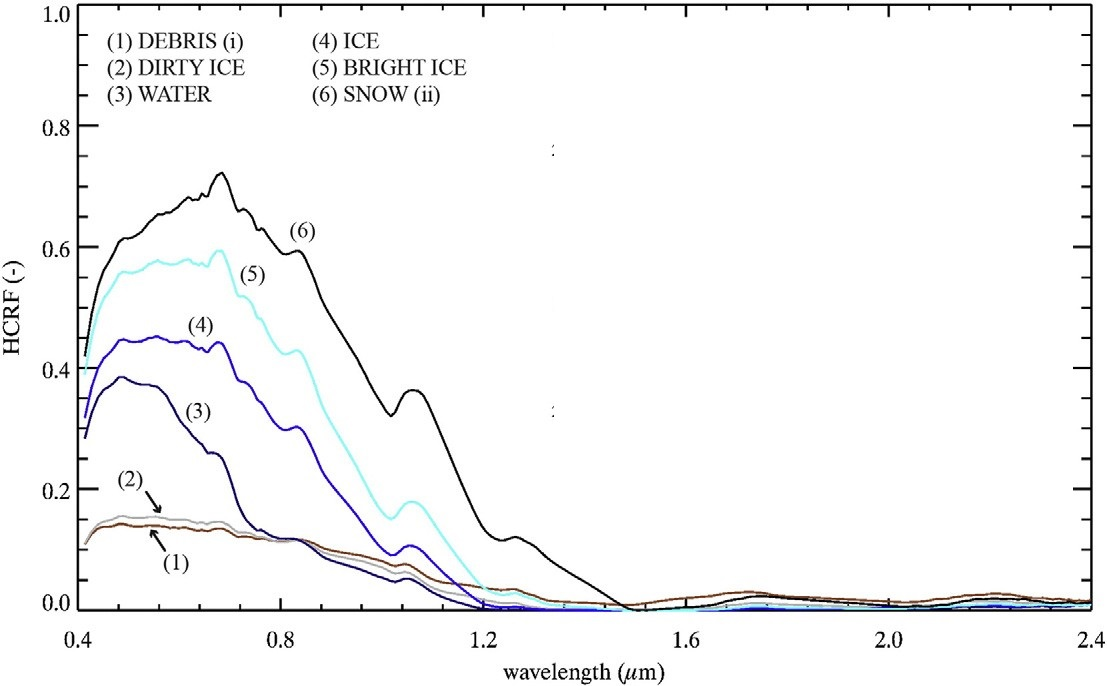
\includegraphics[width=0.50\textwidth]{figures/Orbiter/ice_surface_assessment_spectra}
\caption{An overview of six different ice spectra. Adapted from:\cite{naegeli2015a}.}
\label{fig:ice_assessment_spectra}
\end{figure}

The second paper focuses on assessment of snow and glaciers using imaging spectroscopy\cite{negi2015a}. The spectra in figure (\ref{fig:ice_assessment_spectra2}) illustrates the change in reflectance, when the ice is contaminated with soil, ash or coal and the different reflectance, when the surface has different features. It can be seen how most of the critical spectral data identifying the specific glacial surface is found within the visible region, 400 to 1000 nm, as shown in Figure \ref{fig:ice_spectra_contamination}.
\begin{figure}[htb!]
    \centering
    \captionsetup[subfigure]{width=0.45\textwidth}
    \subfloat[Particle contamination]{
        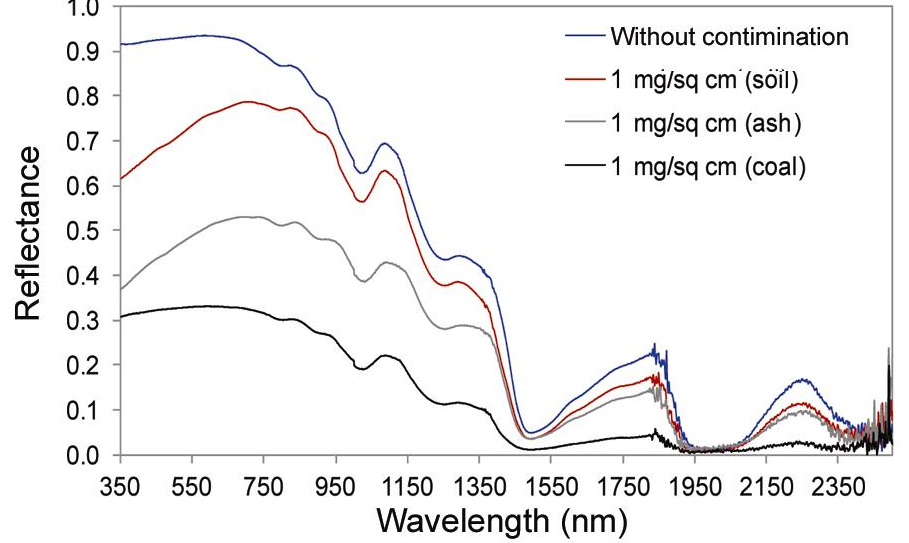
\includegraphics[width=.48\textwidth]{figures/Orbiter/ice_surface_assessment_spectra_contamination}
        \label{fig:ice_spectra_contamination}
    }
    \subfloat[Ice composition]{
        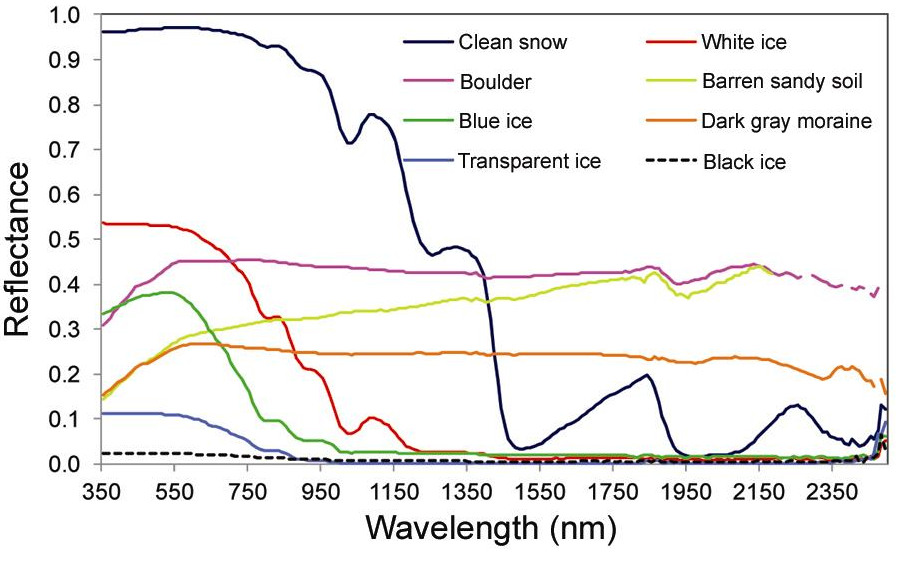
\includegraphics[width=.48\textwidth]{figures/Orbiter/ice_surface_assessment_spectra_feature}
        \label{fig:ice_spectra_feature}
    }
    \caption{A set of example spectra illustrating a contaminated ice surface. Source:\cite{negi2015a}.}\label{fig:ice_assessment_spectra2}
\end{figure}

\noindent
When using imaging spectroscopy for surface material composition analysis, it is often required to work in the near IR and IR ranges to cover the spectral data identifying the material. This can be seen in fig (\ref{fig:material_assessment_spectra}), where most of the spectral details are found in the near IR and IR ranges.
\begin{figure}[htb!]
\centering
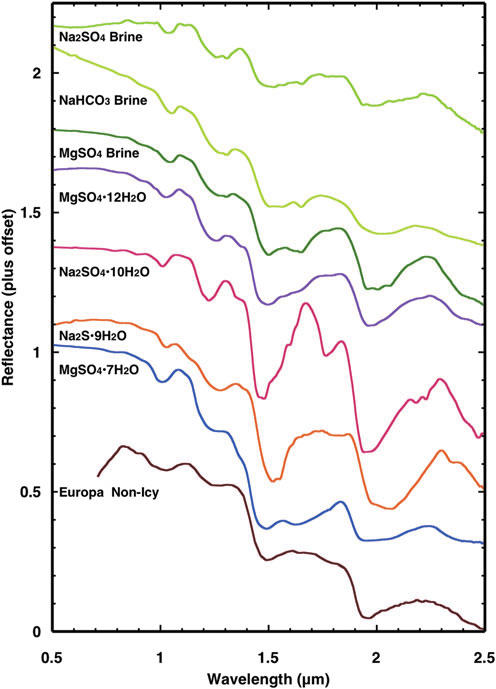
\includegraphics[width=0.5\textwidth]{figures/Orbiter/surface_assessment_sulfate_brine}
\caption{Cryogenic reflectance spectra of hydrated sulfates and brines when observed in the range of 500 nm to 2500 nm (visible and near IR), compared to Europa non-icy surface. Source:\cite{pappalardo2013a}.}
\label{fig:material_assessment_spectra}
\end{figure}
The detector and therefore the imaging spectrometer is expected to capture within the visible region, from approximately 400 to 1000 nm. This limits the usability for the spectrometer, unless a detector with better IR capabilities is selected for the design.
\subsection{Data Processing and Storage System}
Due to the limited communication link, the imaging system cannot transfer the raw data directly to the ground station. This would also be very inefficient, as only a small part of the data will be needed to select a suitable landing site. Therefore, the imaging system requires a data processing system to reorder, store and filter the data, before they are transferred to the ground station. This concept is illustrated in figure (\ref{fig:dat_process_concept}). The processing stage performs a set of six different tasks.
\begin{figure}[htb!]
\centering
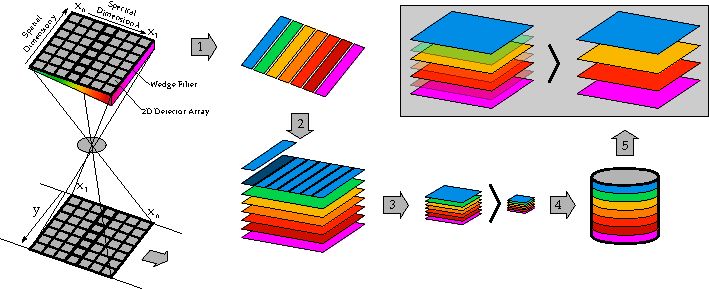
\includegraphics[width=\textwidth]{figures/Orbiter/data_processing_system.pdf}
\caption{The Data Processing and Storage concept.}
\label{fig:dat_process_concept}
\end{figure}
\begin{description}
\item[1. Accumulate] First, the data must be collected from the sensors. Each spectral line has a row of pixels associated with it. Each row should therefore be grouped according to the spectral band.
\item[2. Reorder] When the data are collected from the detector, they will be arranged in spectral \textit{lines}. It is important to keep in mind, that each spectral band will cover a different surface area. Therefore, it will take some time before a specific area has been scanned by all the filters, effectively delaying the time until the spectral sheet has been processed completely. While the data could be stored in the order they are received, this would make the selection process very complicated, as the data must be rearranged each time data are requested by the ground station. Therefore, it makes more sense to accumulate, reorder and store - before the ground station will receive or select the data.
\item[3. Compress] To minimise the load on the storage and communication system, all data should be compressed. It is likely that this part of the imaging system will be shared with the remaining systems on the orbiter.
\item[4. Store] When a set of spectral sheets has been accumulated and compressed, they can be stored in the solid state storage. At this point, it is unknown how much space that will be required. However, it is expected that the storage must be large enough to hold all scanned spectra, even if they are not needed for the landing site selection. After the landing is complete, the less important data can be transmitted as they are still very valuable for scientists and future missions.
\item[5. Select] When all areas has been covered, the ground station can request the specific data that will be relevant for the landing site selection. All collected data will be stored but only the selected data will be transmitted back to the ground station. In this way, the communication capacity can used efficiently. 
\end{description}
All of the required tasks are very suitable for a parallel design, as each spectral data stream can be individually processed. It is likely that the image processing system will be implemented on an FPGA or ASIC, due to the excellent parallel performance that can be obtained, unlike a generic processor. 
Naturally, most of the tasks will be very specific for the image system and will be difficult to reuse for the other systems. However, the image system provides both a storage system and a compression system that can be shared with the remaining systems. It is also very likely, that the image processing module will be paired with a general purpose programmable CPU as not all tasks are suited for an FPGA or ASIC implementation. Naturally, this CPU can be shared with the other systems as well.
%\todo[inline]{overall block diagram of the data processing system data widths}
\subsection{Storage Estimates}
A major part of the processing system revolves around the data storage design. The image system generates large quantities of data so it is necessary to get an estimate of how much data storage that is needed for the final design. Referring to the sensor parameters listed in table (\ref{tab:ccd_calc_parameters}), the first step is to calculate the data generated each time a frame is captured. When capturing an image from a sensor, the analog voltage from each pixel is converted into a digital value. It is expected that a resolution of more than 8 bits will required to provide adequate pixel resolution but more than 16 bits is not very likely, mainly due to the vast amount of data that will be generated. While an FPGA or ASIC implementation of the image processing system can process "odd" data widths, the data must be rounded to even bytes when they are stored. Therefore, 16 bits has been selected as the worst case scenario, resulting in two bytes per pixel. Using the previous sensor parameters, this results in $\approx 2 Mbytes$ per image frame.
%\todo[inline]{Remember to refer to this worst case calculation! The storage requirements can be decreased by half, taking this in account.}
\begin{table}[htb!]
  \centering
\begin{tabular}{l|r|r|l}
\textit{\textbf{Image Frame Data}} & \textit{Minimum} & \multicolumn{1}{r}{\textit{Maximum}} &  \bigstrut[b]\\
\cline{1-3}\textbf{ADC Resolution} & 8     & 16    & [bits] \bigstrut[t]\\
\textbf{Rounded} & 1     & 2     & [bytes] \bigstrut[b]\\
\cline{1-3}\textbf{Image Resolution} & 1048576 & 1048576 & [pixels] \bigstrut\\
\cline{1-3}\textbf{Raw Data Generated} & 1048576 & 2097152 & [bytes] \bigstrut[t]\\
      & 1.048576 & 2.097152 & [mbytes] \\
      & 0.001048576 & 0.002097152 & [gbytes] \\
\end{tabular}%
    \caption{The expected data required for storing each raw image frame.}
  \label{tab:img_frame_data}%
\end{table}%
The next step is to determine how often images must be captured to ensure each area is covered exactly once. First, it is assumed that a full frame is captured of the surface, i.e. no spectral imaging. The parameters used for the calculations are found in table (\ref{tab:imaging_parameters}). The ground distance ($gdist$) is calculated from the resolution per pixel ($mpp$) by multiplying by the number of pixels in each direction, as specified in table (\ref{tab:ccd_calc_parameters}).
\begin{table}[htb!]
  \centering
    \begin{tabular}{l|l|r|r|l}
\textit{\textbf{Parameters}} & \textit{Abbreviation} & \multicolumn{1}{r}{\textit{WAC}} & \multicolumn{1}{r}{\textit{NAC}} &  \bigstrut[b]\\
\cline{1-4}\textbf{Far Distance} & $dist_{far}$ & \multicolumn{2}{c|}{2000.00} & [km] \bigstrut[t]\\
\textbf{Near Distance} & $dist_{near}$ & \multicolumn{2}{c|}{100.00} & [km] \\
\textbf{Average Velocity} & $V_{avg}$ & \multicolumn{2}{c|}{3.30} & [km/s] \bigstrut[b]\\
\cline{1-4}\textbf{Resolution, far} & $mpp_{far,x}$ & 100.00 & 10.00 & [m/pixel] \bigstrut[t]\\
      & $mpp_{far,y}$ & 100.00 & 10.00 & [m/pixel] \bigstrut[b]\\
\cline{2-4}\textbf{Resolution, near} & $mpp_{near,x}$ & 5.00  & 0.50  & [m/pixel] \bigstrut[t]\\
      & $mpp_{near,y}$ & 5.00  & 0.50  & [m/pixel] \bigstrut[b]\\
\cline{1-4}\textbf{Ground Dist, far} & $gdist_{far,x}$ & 102400.00 & 10240.00 & [m] \bigstrut[t]\\
      & $gdist_{far,y}$ & 102400.00 & 10240.00 & [m] \bigstrut[b]\\
\cline{2-4}\textbf{Ground Dist, near} & $gdist_{near,x}$ & 5120.00 & 512.00 & [m] \bigstrut[t]\\
      & $gdist_{near,y}$ & 5120.00 & 512.00 & [m] \\
\end{tabular}%
  \caption{The orbit and ground parameters used.}
  \label{tab:imaging_parameters}%
\end{table}%
Using the orbit parameters and the ground distances provided, the maximum imaging interval can be calculated. It is expected that the ground area covered by the imaging system will move with the same average velocity as the orbiter, $3300 [m/s]$. Knowing the ground velocity, the ground distances can be used to calculate the maximum imaging interval (in seconds) that is required to ensure the surface will be covered (\ref{eq:imaging_interval_calc}). From the interval, the frame rate can be derived (\ref{eq:imaging_rate_calc}) by the reciprocal value. The imaging interval is essentially the maximum available shutter time until the next image must be captured. The ground distance at the far range is used in the below equations.
\begin{equation}\label{eq:imaging_interval_calc}
\tau_{far} = \frac{gdist_{far,WAC}}{V_{avg}} = \frac{104857.6[m]}{3300[m/s]} = 31.775 [s]
\end{equation}
\begin{equation}\label{eq:imaging_rate_calc}
fps_{far} = \frac{1}{gdist_{far,WAC}/V_{avg}} = \frac{1}{104857.6[m]/3300[m/s]} = 0.031 [fps]
\end{equation}
\begin{table}[htb!]
  \centering
\begin{tabular}{l|l|r|r|l}
\textit{\textbf{Imaging Intervals}} & \textit{Abbreviation} & \multicolumn{1}{r}{\textit{WAC}} & \multicolumn{1}{r}{\textit{NAC}} &  \bigstrut[b]\\
\cline{1-4}\textbf{Far (2000km)} & $\tau_{far}$ & 31.030 & 3.103 & [sec] \bigstrut[t]\\
      & $fps_{far}$ & 0.032 & 0.322 & [fps] \bigstrut[b]\\
\cline{1-4}\textbf{Close (100km)} & $\tau_{near}$ & 1.552 & 0.155 & [sec] \bigstrut[t]\\
      & $fps_{near}$ & 0.645 & 6.445 & [fps] \bigstrut[b]\\
\cline{1-4}\textbf{Data Rate, far} & $rate_{far}$ & 0.068 & 0.676 & [MB/s] \bigstrut[t]\\
\textbf{} & -     & 0.000 & 0.001 & [GB/s] \bigstrut[b]\\
\cline{2-4}\textbf{Data Rate, near} & $rate_{near}$ & 1.352 & 13.517 & [MB/s] \bigstrut[t]\\
\textbf{} & -     & 0.001 & 0.014 & [GB/s] \\
\end{tabular}%
      \caption{The maximum imaging intervals and frame rates expected.}
  \label{tab:imaging_interval}%
\end{table}%
The resulting imaging intervals are shown in table (\ref{tab:imaging_interval}), for both cameras. The data rate per second can then be determined from the frame rate, by multiplication, according to table (\ref{tab:img_frame_data}). It can be seen how the data rate is relatively low for both cameras, when capturing full frames.

Using the same method, the frame rates and data rates can be calculated at all distances, as listed in table (\ref{tab:rate_vs_dist_wac}), (\ref{tab:rate_vs_dist_nac}) and compared in figure (\ref{fig:imaging_data_rate_dist_compare}). The ground resolution $mpp$ and ground distance $gdist$ is also calculated for all distances.
% Table generated by Excel2LaTeX from sheet 'Ark1'
\begin{table}[htb!]
  \centering
    \begin{tabular}{l|r|r|r|r|}
\multicolumn{3}{c|}{\textit{\textbf{WAC Rate vs. Distance}}} & \multicolumn{1}{r}{\textit{\textbf{}}} &  \bigstrut[b]\\
\cline{1-3}\textbf{[km]} & \textit{Res. [m/pix]} & \multicolumn{1}{c|}{\textit{Ground [m]}} & \multicolumn{1}{c}{\textit{Frame Rate [fps]}} & \textit{Data Rate [MB/s]} \bigstrut\\
\hline
\textbf{2000} & 100.0 & 102400.0 & 0.032 & 0.068 \bigstrut[t]\\
\textbf{1750} & 87.5  & 89600.0 & 0.037 & 0.077 \\
\textbf{1500} & 75.0  & 76800.0 & 0.043 & 0.090 \\
\textbf{1250} & 62.5  & 64000.0 & 0.052 & 0.108 \\
\textbf{1000} & 50.0  & 51200.0 & 0.064 & 0.135 \\
\textbf{800} & 40.0  & 40960.0 & 0.081 & 0.169 \\
\textbf{400} & 20.0  & 20480.0 & 0.161 & 0.338 \\
\textbf{200} & 10.0  & 10240.0 & 0.322 & 0.676 \\
\textbf{100} & 5.0   & 5120.0 & \textbf{0.645} & \textbf{1.352} \\
\end{tabular}%
    \caption{The data rate vs. the distance, when operating the WAC in full frame mode.}
  \label{tab:rate_vs_dist_wac}%
\end{table}%
% Table generated by Excel2LaTeX from sheet 'Ark1'
\begin{table}[htb!]
  \centering
    \begin{tabular}{r|r|r|r|r|}
\multicolumn{3}{c|}{\textit{\textbf{NAC Rate vs. Distance}}} & \multicolumn{1}{r}{\textit{\textbf{}}} &  \bigstrut[b]\\
\cline{1-3}\textbf{[km]} & \textit{Res. [m/pix]} & \multicolumn{1}{c|}{\textit{Ground [m]}} & \multicolumn{1}{c}{\textit{Frame Rate [fps]}} & \textit{Data Rate [MB/s]} \bigstrut\\
\hline
\textbf{2000} & 10.0  & 10240.0 & 0.322 & 0.676 \bigstrut[t]\\
\textbf{1750} & 8.8   & 8960.0 & 0.368 & 0.772 \\
\textbf{1500} & 7.5   & 7680.0 & 0.430 & 0.901 \\
\textbf{1250} & 6.3   & 6400.0 & 0.516 & 1.081 \\
\textbf{1000} & 5.0   & 5120.0 & 0.645 & 1.352 \\
\textbf{800} & 4.0   & 4096.0 & 0.806 & 1.690 \\
\textbf{400} & 2.0   & 2048.0 & 1.611 & 3.379 \\
\textbf{200} & 1.0   & 1024.0 & 3.223 & 6.758 \\
\textbf{100} & 0.5   & 512.0 & \textbf{6.445} & \textbf{13.517} \\
\end{tabular}%
    \caption{The data rate vs. the distance, when operating the NAC in full frame mode.}
  \label{tab:rate_vs_dist_nac}%
\end{table}%
\begin{figure}[htb!]
\centering
\includegraphics[width=0.5\textwidth,page=3,trim=15mm 15mm 15mm 32mm,clip]{figures/Orbiter/Graphs_excel.pdf}
\caption{The data rate relative to the distance, when no spectrometer is used.}
\label{fig:imaging_data_rate_dist_compare}
\end{figure}
\begin{figure}[htb!]
\centering
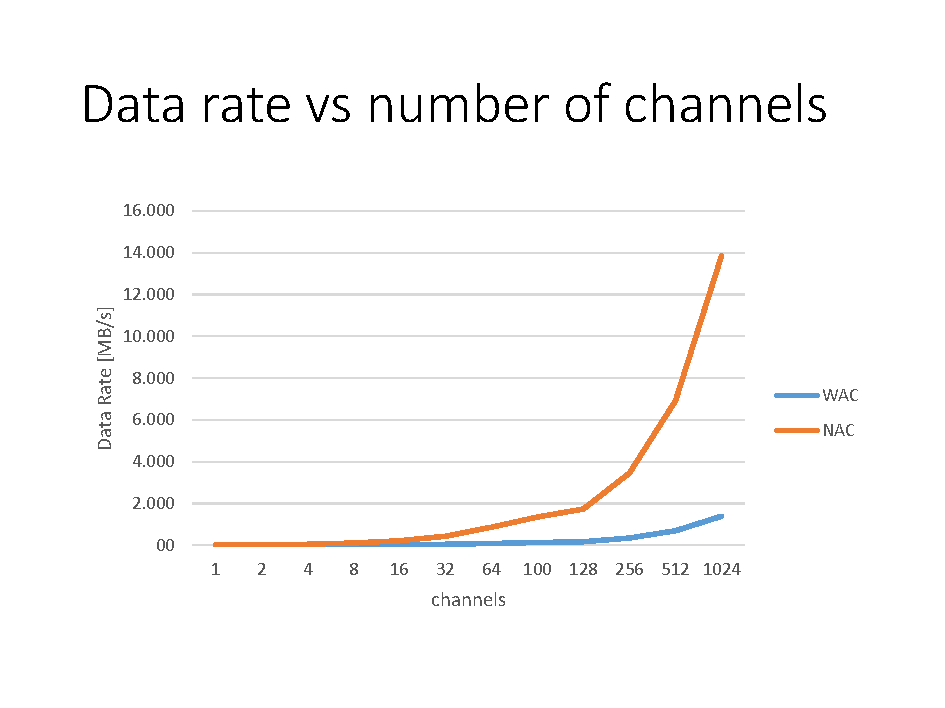
\includegraphics[width=0.5\textwidth,page=1,trim=15mm 15mm 15mm 32mm,clip]{figures/Orbiter/Graphs_excel.pdf}
\caption{The data rate relative to the number of spectral channels, at the closest distance.}
\label{fig:imaging_data_rate_growth}
\end{figure}
The next step is to determine the data rate, when a spectrometer is added to the system. As the number of spectral channels is not known at this point, the data rate growth will be determined to select a suitable number of channels. Naturally, it is always necessary to image the surface with no filters applied. Therefore, it is expected that one of the channels will not be covered by the wedge filter, essentially imaging the surface as a push broom imager, while capturing spectral data as well.

For these calculations, the worst case situation, the closest distance (100 km), is selected, as the imaging system will operate at the highest rate. When the number of spectral channels is increased, less pixel rows are used per channel, effectively reducing the ground distance covered by the imager. A lower ground distance will naturally result in a higher frame rate and therefore a higher data rate, as calculated by (\ref{eq:imaging_rate_calc}). The data rate growth is shown in table (\ref{tab:imaging_data_rate_growth}) and figure (\ref{fig:imaging_data_rate_growth}).
\begin{table}[htb!]
  \centering
  \resizebox{\textwidth}{!}{%
    \begin{tabular}{l|r|r|r|r|r|r|r|}
\textit{\textbf{}} & \textit{Pixel Rows} & \multicolumn{2}{c|}{\textit{Ground Dist [m]}} & \multicolumn{2}{c|}{\textit{Frame Rate [fps]}} & \multicolumn{2}{c}{\textit{Data Rate [MB/s]}} \bigstrut[b]\\
\cline{1-1}\textbf{CH\tablefootnote{Number of spectral channels in operation.}} & \textit{WAC, NAC} & \textit{WAC} & \textit{NAC} & \textit{WAC} & \textit{NAC} & \textit{WAC} & \multicolumn{1}{r}{\textit{NAC}} \bigstrut\\
\hline
\textbf{1} & 1024  & 5120.0 & 512.0 & 0.6   & 6.4   & 1.4   & 13.5 \bigstrut[t]\\
\textbf{2} & 512   & 2560.0 & 256.0 & 1.3   & 12.9  & 2.7   & 27.0 \\
\textbf{4} & 256   & 1280.0 & 128.0 & 2.6   & 25.8  & 5.4   & 54.1 \\
\textbf{8} & 128   & 640.0 & 64.0  & 5.2   & 51.6  & 10.8  & 108.1 \\
\textbf{16} & 64    & 320.0 & 32.0  & 10.3  & 103.1 & 21.6  & 216.3 \\
\textbf{32} & 32    & 160.0 & 16.0  & 20.6  & 206.3 & 43.3  & 432.5 \\
\textbf{64} & 16    & 80.0  & 8.0   & 41.3  & 412.5 & 86.5  & 865.1 \\
\textbf{100} & 10    & 51.2  & 5.1   & 64.5  & 644.5 & 135.2 & 1351.7 \\
\textbf{128} & 8     & 40.0  & 4.0   & 82.5  & 825.0 & 173.0 & 1730.2 \\
\textbf{256} & 4     & 20.0  & 2.0   & 165.0 & 1650.0 & 346.0 & 3460.3 \\
\textbf{512} & 2     & 10.0  & 1.0   & 330.0 & 3300.0 & 692.1 & 6920.6 \\
\textbf{1024} & 1     & 5.0   & 0.5   & 660.0 & 6600.0 & 1384.1 & 13841.2 \\
\end{tabular}}%
    \caption{The data rate growth at 100 km, varying spectrometer channels.}
  \label{tab:imaging_data_rate_growth}%
\end{table}%
From these results, it is clear that adding a spectrometer will generate a much larger amount of data - especially for the NAC due to its already high resolution. Also important to notice is the huge frame rate required when operating at a high number of channels. This is an obvious issue when operating the wedge spectrometer in push broom mode. If the whisk broom is selected instead, the effective frame rate will be reduced significantly however the coverage will be reduced as well. High coverage per flyby is important in this design so changing to whisk broom mode is not an option.

However, it is very unlikely that the spectral data for very high ground resolutions ($<5[m/pixel]$) and very low ground resolutions ($>50[m/pixel]$) will be relevant for the landing site selection. By reducing the spectral resolution when operating outside these regions, the generated data can be reduced significantly. From figure (\ref{fig:imaging_data_rate_growth}), it is clear that the data rate increases rapidly at higher channel numbers. For the remaining calculations, 100 spectral channels has been selected as this balances a high spectral resolution with a sensible frame and data rate.
\begin{table}[htb!]
  \centering
  \resizebox{\textwidth}{!}{%
    \begin{tabular}{l|r|r|r|r|r|}
\multicolumn{4}{c|}{\textit{\textbf{WAC Rate Growth vs. Distance}}} & \multicolumn{1}{r}{} & \multicolumn{1}{r}{} \bigstrut[b]\\
\cline{1-4}\textbf{[km]} & \textit{CH} & \textit{Res. [m/pix]} & \multicolumn{1}{c|}{\textit{Ground [m]}} & \multicolumn{1}{c}{\textit{Frame Rate [fps]}} & \multicolumn{1}{r}{\textit{Data Rate [MB/s]}} \bigstrut\\
\hline
\textbf{2000} & 1     & 100.00 & 102400.00 & 0.03  & 0.07 \bigstrut[t]\\
\textbf{1750} & 1     & 87.50 & 89600.00 & 0.04  & 0.08 \\
\textbf{1500} & 1     & 75.00 & 76800.00 & 0.04  & 0.09 \\
\textbf{1250} & 1     & 62.50 & 64000.00 & 0.05  & 0.11 \\
\textbf{1000} & 100   & 50.00 & 512.00 & 6.45  & 13.52 \\
\textbf{800} & 100   & 40.00 & 409.60 & 8.06  & 16.90 \\
\textbf{400} & 100   & 20.00 & 204.80 & 16.11 & 33.79 \\
\textbf{200} & 1     & 10.00 & 10240.00 & 0.32  & 0.68 \\
\textbf{100} & 1     & 5.00  & 5120.00 & \textbf{0.64} & \textbf{1.35} \\
\end{tabular}}%
  \caption{The rate growth for the WAC, when optimal spectral resolution is selected.}
  \label{tab:opt_rate_growth_wac}%
\end{table}%
 The rate growth calculations has been repeated for the WAC and the NAC, this time using optimal spectral resolutions. The spectral resolution has been selected depending on the ground resolution and therefore the distance. It is expected that the spectrometer will either be operating at the 
\begin{table}[htb!]
  \centering
    \begin{tabular}{l|r|r|r|r|r|}
\multicolumn{4}{c|}{\textit{\textbf{NAC Rate Growth vs. Distance}}} & \multicolumn{1}{r}{} & \multicolumn{1}{r}{} \bigstrut[b]\\
\cline{1-4}\textbf{[km]} & \textit{CH} & \textit{Res. [m/pix]} & \multicolumn{1}{c|}{\textit{Ground [m]}} & \multicolumn{1}{c}{\textit{Frame Rate [fps]}} & \multicolumn{1}{r}{\textit{Data Rate [MB/s]}} \bigstrut\\
\hline
\textbf{2000} & 100   & 10.00 & 102.40 & 32.23 & 67.58 \bigstrut[t]\\
\textbf{1750} & 100   & 8.75  & 89.60 & 36.83 & 77.24 \\
\textbf{1500} & 100   & 7.50  & 76.80 & 42.97 & 90.11 \\
\textbf{1250} & 100   & 6.25  & 64.00 & 51.56 & 108.13 \\
\textbf{1000} & 100   & 5.00  & 51.20 & \textbf{64.45} & \textbf{135.17} \\
\textbf{800} & 1     & 4.00  & 4096.00 & 0.81  & 1.69 \\
\textbf{400} & 1     & 2.00  & 2048.00 & 1.61  & 3.38 \\
\textbf{200} & 1     & 1.00  & 1024.00 & 3.22  & 6.76 \\
\textbf{100} & 1     & 0.50  & 512.00 & 6.45  & 13.52 \\
\end{tabular}%
  \caption{The rate growth for the NAC, when optimal spectral resolution is selected.}
  \label{tab:opt_rate_growth_nac}%
\end{table}%
The results are found in table (\ref{tab:opt_rate_growth_wac}) and (\ref{tab:opt_rate_growth_nac}). It can be seen how both cameras will be operating as a spectrometer; the WAC uses the spectrometer mainly at the closer distances while the NAC operates at the far distances. This ensures the spectrometer is only operated, when the ground resolution is within a range of $5[m/pixel]$ to $50[m/pixel]$. This keeps the data- and frame rate within sensible limits, avoiding the costs of specialised very high speed image sensors and processing systems. However, from a design point of view, the data rates are still high. 

Combining the data rate from the WAC and the NAC, the peak data rates that must be handled by the processing system can be calculated. The result is shown in table (\ref{tab:peak_data_wac_nac}). The peak data rates has been illustrated in figure (\ref{fig:imaging_data_peak_throughput}).
\begin{table}[htb!]
  \centering
    \begin{tabular}{l|r|r|r|}
\textit{\textbf{Peak data rate, WAC + NAC}} & \multicolumn{3}{c|}{\textit{Data Rate [MB/s]}} \bigstrut[b]\\
\cline{1-1}\textbf{[km]} & \textit{WAC} & \textit{NAC} & \multicolumn{1}{c|}{\textit{Total}} \bigstrut\\
\hline
\textbf{2000} & 0.07  & \multicolumn{1}{r}{67.58} & 67.65 \bigstrut[t]\\
\textbf{1750} & 0.08  & \multicolumn{1}{r}{77.24} & 77.32 \\
\textbf{1500} & 0.09  & \multicolumn{1}{r}{90.11} & 90.20 \\
\textbf{1250} & 0.11  & \multicolumn{1}{r}{108.13} & 108.24 \\
\textbf{1000} & 13.52 & \multicolumn{1}{r}{135.17} & \textbf{148.68} \\
\textbf{800} & 16.90 & \multicolumn{1}{r}{1.69} & 18.59 \\
\textbf{400} & 33.79 & \multicolumn{1}{r}{3.38} & 37.17 \\
\textbf{200} & 0.68  & \multicolumn{1}{r}{6.76} & 7.43 \\
\textbf{100} & 1.35  & \multicolumn{1}{r}{13.52} & 14.87 \\
\end{tabular}%
    \caption{The combined data rate from the WAC and the NAC}
  \label{tab:peak_data_wac_nac}%
\end{table}%
\begin{figure}[htb!]
%left bottom right top
\centering
\includegraphics[width=0.6\textwidth,page=2,trim=15mm 15mm 15mm 32mm,clip]{figures/Orbiter/Graphs_excel.pdf}
\caption{The peak data rate, using 100 spectrometer channels at specific distances.}
\label{fig:imaging_data_peak_throughput}
\end{figure}

\noindent
This method assumes that it is possible to switch from full frame mode to spectral mode, either by switching the detector or wedge filter. Reducing the spectral resolution instead may be possible instead, if the processing system and the sensor supports reading and storing individual rows.

For the final part of the analysis, the expected ground coverage and the accumulated data generated has be calculated. This will give a good idea of imaging system performance and the requirements from the processing system. First, it is necessary to calculate the expected flyby time. For this estimate, a linear approximation of the flyby is used. This concept is illustrated in figure (\ref{fig:linear_flyby}). 
\begin{figure}[htb!]
%left bottom right top
\centering
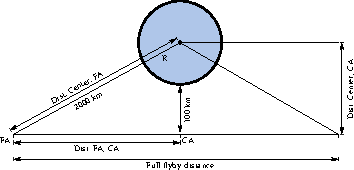
\includegraphics[width=0.6\textwidth]{figures/Orbiter/linear_flyby.pdf}
\caption{The linear approximation of the flyby.}
\label{fig:linear_flyby}
\end{figure}
Europa is here illustrated by the blue circle. The flyby parameters used are listed in table (\ref{tab:orbit_parameters_linear}). A constant average velocity has been used for the full flyby. While this is not completely accurate, it still gives a good estimate of the required flyby duration.%The average velocity has been changed according to the actual flyby proposed earlier in this report. 
The flyby is expected to go from furthest approach (FA) to closest approach (CA) and then finally back to (FA).
\begin{table}[htb!]
  \centering
    \begin{tabular}{l|l|r|l}
\textit{\textbf{Flyby Parameters}} & \textit{Abbreviation} & \multicolumn{1}{r}{\textit{Value}} &  \bigstrut[b]\\
\cline{1-3}\textbf{Closest Approach} & CA    & 100.00 & [km] \bigstrut[t]\\
\textbf{Furthest Approach} & FA    & 2000.00 & [km] \\
\textbf{Europa Radius} & R     & 1560.00 & [km] \\
\textbf{Avg Velocity} & $V_{avg}$ & 3.30  & [km/s] \\
\textbf{Europa Surface Area} & $A_{eu}$ & 30900000.00 & [$km^2$] \\
\end{tabular}%
    \caption{The orbit parameters used for the linear approximation.}
  \label{tab:orbit_parameters_linear}%
\end{table}%

Using these orbit parameters, the total flyby distance and time can be calculated. Referring to figure (\ref{fig:linear_flyby}), the distance between FA and CA can be calculated, using the distance between CA, FA and the center of Europa (\ref{eq:dist_centers}):
\begin{equation}\label{eq:dist_centers}
\begin{split}
dist_{cen,FA} &= FA+R\\
dist_{cen,CA} &= CA+R\\
\end{split}
\end{equation}
The distance between FA and CA is now calculated, resulting in the linear flyby distance.
\begin{equation}\label{eq:dist_fa_ca}
dist_{FA, CA} = \sqrt{dist_{cen,FA}^2-dist_{cen,CA}^2} \rightarrow
\end{equation}
\begin{equation}\label{eq:dist_flyby_dist}
dist_{flyby} = 2\cdot dist_{FA, CA}
\end{equation}
The flyby duration can then be determined, using the average velocity:
\begin{equation}
T_{flyby,s} = \frac{dist_{flyby}}{V_{avg}}
\end{equation}
\begin{table}[htb!]
  \centering
    \begin{tabular}{l|l|r|l}
\textit{\textbf{Initial Conditions}} & \textit{Abbreviation} & \multicolumn{1}{r}{\textit{Value}} &  \bigstrut[b]\\
\cline{1-3}\textbf{Dist. Center, FA} & $dist_{cen,FA}$ & 3560.00 & [km] \bigstrut[t]\\
\textbf{Dist. Center, CA} & $dist_{cen,CA}$ & 1660.00 & [km] \bigstrut[b]\\
\cline{1-3}\textbf{Dist. FA, CA} & $dist_{FA, CA}$ & 3149.29 & [km] \bigstrut[t]\\
\textbf{Flyby Distance} & $dist_{flyby}$ & 6298.57 & [km] \bigstrut[b]\\
\cline{1-3}\textbf{Flyby Duration} & $T_{flyby,s}$ & 1908.66 & [s] \bigstrut[t]\\
      & $T_{flyby,m}$ & \textbf{31.81} & [m] \\
\end{tabular}%
  \caption{The details of the flyby. A flyby of approximately 31 minutes is estimated.}
  \label{tab:flyby_init_cond}%
\end{table}%

\noindent
The resulting initial conditions for the flyby are found in table (\ref{tab:flyby_init_cond}). From this, the linear approximation of the flyby can be used to calculate the amount of data that will be generated during one flyby. The distance to CA changes, as the spacecraft moves. The new distance is calculated from the current velocity and the time it takes to get there, according to (\ref{eq:fa_to_ca}).
\begin{equation}\label{eq:fa_to_ca}
dist_{CA} = dist_{CA,prev}-V_{avg}\cdot T_{flyby,s}
\end{equation}
The altitude can now be calculated using the values already known (\ref{eq:altitude}), according to figure (\ref{fig:linear_flyby_move}).
\begin{equation}\label{eq:altitude}
altitude = \sqrt{dist_{cen,CA}^2+dist_{CA}^2}-R
\end{equation}
\begin{figure}[htb!]
\centering
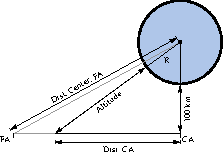
\includegraphics[width=0.6\textwidth]{figures/Orbiter/linear_flyby_move.pdf}
\caption{Calculating the new position.}
\label{fig:linear_flyby_move}
\end{figure}
By calculating the ground distance according to the altitude, as it was done in table \ref{tab:rate_vs_dist_wac}, the imaging rate can then be calculated according to equation (\ref{eq:imaging_rate_calc}). The total number of frames can then be calculated from the time between the two intervals and the frame rate. The total data generated during an interval and a flyby is also calculated using this way. The results are shown in table (\ref{tab:wac_flyby_data}).
\begin{table}[htb!]
  \centering
  \resizebox{\textwidth}{!}{%
    \begin{tabular}{l|r|r|r|r|r|r|r|r|}
      & \textit{Time} & \textit{Dist. CA} & \textit{Altitude} & \multicolumn{1}{c|}{\textit{Frames}} & \textit{Frames} & \textit{Data} & \multicolumn{2}{c}{\textit{Total Data [MB]}} \\
\textbf{I} & \textit{[s]} & \textit{[km]} & \textit{[km]} & \textit{[fps]} & \textit{interval} & \textit{[MB/s]} & \textit{Interval} & \multicolumn{1}{r}{\textit{Flyby}} \bigstrut[b]\\
\hline
\textbf{0} & 0.00  & 3149.29 & 2000.00 & 0.032 & 6.15  & 0.068 & 12.90 & 12.90 \bigstrut[t]\\
\textbf{1} & 190.87 & 2519.43 & 1457.14 & 0.044 & 8.44  & 0.093 & 17.71 & 30.60 \\
\textbf{2} & 381.73 & 1889.57 & 955.17 & 0.067 & 12.88 & 0.142 & 27.01 & 57.61 \\
\textbf{3} & 572.60 & 1259.71 & 523.86 & 0.123 & 23.48 & 0.258 & 49.25 & 106.86 \\
\textbf{4} & 763.46 & 629.86 & 215.48 & 0.299 & 57.09 & 0.627 & 119.73 & 226.59 \\
\textbf{5} & 954.33 & 0.00  & 100.00 & 0.645 & 123.02 & 1.352 & 257.99 & 484.58 \\
\textbf{6} & 1145.19 & -629.86 & 215.48 & 0.299 & 57.09 & 0.627 & 119.73 & 604.31 \\
\textbf{7} & 1336.06 & -1259.71 & 523.86 & 0.123 & 23.48 & 0.258 & 49.25 & 653.56 \\
\textbf{8} & 1526.93 & -1889.57 & 955.17 & 0.067 & 12.88 & 0.142 & 27.01 & 680.57 \\
\textbf{9} & 1717.79 & -2519.43 & 1457.14 & 0.044 & 8.44  & 0.093 & 17.71 & 698.27 \\
\textbf{10} & 1908.66 & -3149.29 & 2000.00 & 0.032 & 6.15  & 0.068 & 12.90 & \textbf{711.17} \\
\end{tabular}}%
      \caption{The total data produced during a single flyby, using the WAC.}
  \label{tab:wac_flyby_data}%
\end{table}%
It can be seen how around a GB is generated per flyby from the WAC. However, to put the data load in perspective, it is necessary to consider the surface coverage obtained from these data. The total surface coverage has been calculated in table (\ref{tab:wac_flyby_coverage}).
\begin{table}[htb!]
  \centering
  \resizebox{\textwidth}{!}{%
    \begin{tabular}{l|r|r|r|r|r|r|r|r|}
      & \textit{Time} & \textit{Altitude} & \textit{Frames} & \textit{Dist,v} & \textit{Dist,v} & \multicolumn{2}{c|}{\textit{Area $[km^2]$}} & \multicolumn{1}{r}{\textit{Area}} \\
\textbf{I} & \textit{[s]} & \textit{[km]} & \textit{interval} & \textit{[m]} & \textit{[m]} & \textit{Interval} & \textit{Total} & \multicolumn{1}{r}{\textit{[\%]}} \bigstrut[b]\\
\hline
\textbf{0} & 0.00  & 2000.00 & 6.15  & 102400.0 & 102400.0 & 64497.4 & 64497.4 & 0.21 \bigstrut[t]\\
\textbf{1} & 190.87 & 1457.14 & 8.44  & 74605.5 & 74605.5 & 46990.8 & 111488.1 & 0.57 \\
\textbf{2} & 381.73 & 955.17 & 12.88 & 48904.7 & 48904.7 & 30803.0 & 142291.1 & 1.03 \\
\textbf{3} & 572.60 & 523.86 & 23.48 & 26821.7 & 26821.7 & 16893.9 & 159185.0 & 1.55 \\
\textbf{4} & 763.46 & 215.48 & 57.09 & 11032.4 & 11032.4 & 6948.9 & 166133.8 & 2.08 \\
\textbf{5} & 954.33 & 100.00 & 123.02 & 5120.0 & 5120.0 & 3224.9 & 169358.7 & 2.63 \\
\textbf{6} & 1145.19 & 215.48 & 57.09 & 11032.4 & 11032.4 & 6948.9 & 176307.6 & 3.20 \\
\textbf{7} & 1336.06 & 523.86 & 23.48 & 26821.7 & 26821.7 & 16893.9 & 193201.4 & 3.83 \\
\textbf{8} & 1526.93 & 955.17 & 12.88 & 48904.7 & 48904.7 & 30803.0 & 224004.4 & 4.55 \\
\textbf{9} & 1717.79 & 1457.14 & 8.44  & 74605.5 & 74605.5 & 46990.8 & 270995.2 & 5.43 \\
\textbf{10} & 1908.66 & 2000.00 & 6.15  & 102400.0 & 102400.0 & 64497.4 & 335492.5 & \textbf{6.51} \\
\end{tabular}}%
  \caption{The surface coverage provided during a single flyby, using the WAC.}
  \label{tab:wac_flyby_coverage}%
\end{table}%
With a coverage of $6.51$\% compared to the total area of Europa, at least five flybys will be required before the necessary ground coverage is obtained. However, these estimates all assume the imaging system will pointing in the nadir. No attitude control is used to point the spacecraft at different surface areas, increasing the coverage. Adding this feature would certainly increase the flyby coverage, at the added cost of higher data load. Expecting that the spacecraft will point directly towards a suitable landing site is not realistic. Therefore, it is necessary to increase the ground coverage using attitude control. Repeating the calculations for the NAC results in the data and ground coverage listed in table (\ref{tab:nac_flyby_data}) and (\ref{tab:nac_flyby_data}).
\begin{table}[htb!]
  \centering
  \resizebox{\textwidth}{!}{%
    \begin{tabular}{l|r|r|r|r|r|r|r|r|}
      & \textit{Time} & \textit{Dist. CA} & \textit{Altitude} & \multicolumn{1}{c|}{\textit{Frames}} & \textit{Frames} & \textit{Data} & \multicolumn{2}{c}{\textit{Total [MB]}} \\
\textbf{I} & \textit{[s]} & \textit{[km]} & \textit{[km]} & \textit{[fps]} & \textit{interval} & \textit{[MB/s]} & \textit{Interval} & \multicolumn{1}{r}{\textit{Flyby}} \bigstrut[b]\\
\hline
\textbf{0} & 0.00  & 3149.29 & 2000.00 & 0.322 & 61.51 & 0.676 & 128.99 & 128.99 \bigstrut[t]\\
\textbf{1} & 190.87 & 2519.43 & 1457.14 & 0.442 & 84.43 & 0.928 & 177.05 & 306.05 \\
\textbf{2} & 381.73 & 1889.57 & 955.17 & 0.675 & 128.79 & 1.415 & 270.10 & 576.14 \\
\textbf{3} & 572.60 & 1259.71 & 523.86 & 1.230 & 234.83 & 2.580 & 492.48 & 1068.62 \\
\textbf{4} & 763.46 & 629.86 & 215.48 & 2.991 & 570.91 & 6.273 & 1197.29 & 2265.91 \\
\textbf{5} & 954.33 & 0.00  & 100.00 & 6.445 & 1230.19 & 13.517 & 2579.89 & 4845.81 \\
\textbf{6} & 1145.19 & -629.86 & 215.48 & 2.991 & 570.91 & 6.273 & 1197.29 & 6043.10 \\
\textbf{7} & 1336.06 & -1259.71 & 523.86 & 1.230 & 234.83 & 2.580 & 492.48 & 6535.58 \\
\textbf{8} & 1526.93 & -1889.57 & 955.17 & 0.675 & 128.79 & 1.415 & 270.10 & 6805.68 \\
\textbf{9} & 1717.79 & -2519.43 & 1457.14 & 0.442 & 84.43 & 0.928 & 177.05 & 6982.73 \\
\textbf{10} & 1908.66 & -3149.29 & 2000.00 & 0.322 & 61.51 & 0.676 & 128.99 & \textbf{7111.72} \\
\end{tabular}}%
  \caption{The total data produced during a single flyby, using the NAC.}
  \label{tab:nac_flyby_data}%
\end{table}%
\begin{table}[htb!]
  \centering
  \resizebox{\textwidth}{!}{%
    \begin{tabular}{l|r|r|r|r|r|r|r|r|}
      & \textit{Time} & \textit{Altitude} & \textit{Frames} & \textit{Dist,v} & \textit{Dist,v} & \multicolumn{2}{c|}{\textit{Area $[km^2]$}} & \multicolumn{1}{r}{\textit{Area}} \\
\textbf{I} & \textit{[s]} & \textit{[km]} & \textit{interval} & \textit{[m]} & \textit{[m]} & \textit{Interval} & \textit{Total} & \multicolumn{1}{r}{\textit{[\%]}} \bigstrut[b]\\
\hline
\textbf{0} & 0.00  & 2000.00 & 61.51 & 10240.0 & 10240.0 & 6449.7 & 6449.7 & 0.02 \bigstrut[t]\\
\textbf{1} & 190.87 & 1457.14 & 84.43 & 7460.5 & 7460.5 & 4699.1 & 11148.8 & 0.06 \\
\textbf{2} & 381.73 & 955.17 & 128.79 & 4890.5 & 4890.5 & 3080.3 & 14229.1 & 0.10 \\
\textbf{3} & 572.60 & 523.86 & 234.83 & 2682.2 & 2682.2 & 1689.4 & 15918.5 & 0.15 \\
\textbf{4} & 763.46 & 215.48 & 570.91 & 1103.2 & 1103.2 & 694.9 & 16613.4 & 0.21 \\
\textbf{5} & 954.33 & 100.00 & 1230.19 & 512.0 & 512.0 & 322.5 & 16935.9 & 0.26 \\
\textbf{6} & 1145.19 & 215.48 & 570.91 & 1103.2 & 1103.2 & 694.9 & 17630.8 & 0.32 \\
\textbf{7} & 1336.06 & 523.86 & 234.83 & 2682.2 & 2682.2 & 1689.4 & 19320.1 & 0.38 \\
\textbf{8} & 1526.93 & 955.17 & 128.79 & 4890.5 & 4890.5 & 3080.3 & 22400.4 & 0.46 \\
\textbf{9} & 1717.79 & 1457.14 & 84.43 & 7460.5 & 7460.5 & 4699.1 & 27099.5 & 0.54 \\
\textbf{10} & 1908.66 & 2000.00 & 61.51 & 10240.0 & 10240.0 & 6449.7 & 33549.3 & \textbf{0.65} \\
\end{tabular}}%
  \caption{The surface coverage provided during a single flyby, using the NAC.}
  \label{tab:nac_flyby_coverage}%
\end{table}%

When operating the NAC, the ground coverage will be low but the data load will be very high due to the high resolution of the images. Most of these data are likely to contain scientifically useful data but it is not expected that the data will be transmitted to earth immediately. Only a selection of the high resolution imges will be needed to select a suitable landing site. Therefore, only select few high resolution images will be transmitted, before the landing takes place. After the lander has reached the surface, the remaining high resolution imaging can be transmitted, whenever the communication link is not occupied for more important matters. 

The ground coverage percentage is relatively low but even from one flyby, a surface area of 33549.3$[km^2]$ has been covered by the imager. It is important to keep in mind that the main purpose of the high resolution images is to investigate specific regions further. It is expected that the specific high resolution images that will be selected for further studies will contain interesting regions and possible landing areas. The data rate and amount of accumulated data per flyby has been compared for the two cameras in figure (\ref{fig:data_gen_wac_nac_compare1}).

\begin{figure}[htb!]
    \centering
    \captionsetup[subfigure]{width=0.45\textwidth}
    \subfloat[Data rates]{
        \includegraphics[width=.48\textwidth,page=4,trim=15mm 15mm 15mm 32mm,clip]{figures/Orbiter/Graphs_excel.pdf}
        \label{fig:data_gen_wac_compare}
    }
    \subfloat[Accumulated Data]{
        \includegraphics[width=.48\textwidth,page=5,trim=15mm 15mm 15mm 32mm,clip]{figures/Orbiter/Graphs_excel.pdf}
        \label{fig:data_gen_nac_compare}
    }
    \caption{Comparison between the data rates and accumulated data for both cameras, during each flyby.}\label{fig:data_gen_wac_nac_compare1}
\end{figure}

The coverage can be increased even further if attitude control is used to point the spacecraft. The coverage will then only be limited by the available data storage on the spacecraft. 7111.72$[MB]$ per flyby may sound like a lot, but very large solid state drives (SSDs) already exist and could be used for this purpose. The main constraint is not the storage itself but the available communication capacity. After all, high resolution imaging will be of no use, if they cannot be transmitted within a realistic time frame.

To reduce the storage requirements, it may be necessary for the ground station to discard high resolution images of less interesting surface areas. Whether an area qualifies to be further studied or discarded is a complete different analysis and will not be discussed further in this section.

When recording multi spectral data, the coverage will be the same as the previous examples due to the fact that the system is operated in push broom mode, thus imaging the same ground area. However, the frame rate and therefore the data rate will be significantly increased. The data load will now be calculated, when the spectrometer is added to the system. As before, the WAC will operate within the ground resolution range of around $25[m/pixel]$ to $50[m/pixel]$ whereas the NAC will operate within the ground resolution range of $5[m/pixel]$ to $10[m/pixel]$. Both cases will use all 100 channels. The results are seen in table (\ref{tab:wac_flyby_data_spectrometer}) and (\ref{tab:nac_flyby_data_spectrometer}).
\begin{table}[htb!]
  \centering
  \resizebox{\textwidth}{!}{%
    \begin{tabular}{l|r|r|r|r|r|r|r|r|}
      & \textit{Time} & \textit{CH} & \textit{Altitude} & \textit{Res.} & \textit{Ground} & \textit{Frames } & \multicolumn{2}{c}{\textit{Data}} \\
\textbf{I} & \textit{[s]} & \textit{} & \textit{[km]} & \textit{[m/pix]} & \multicolumn{1}{c|}{\textit{[m]}} & \multicolumn{1}{c|}{\textit{[fps]}} & \textit{[MB/s]} & \multicolumn{1}{r}{\textit{Flyby}} \bigstrut[b]\\
\hline
\textbf{0} & 0.0   & 1     & 2000.0 & 100.0 & 102400.0 & 0.0   & 0.1   & 12.9 \bigstrut[t]\\
\textbf{1} & 190.9 & 1     & 1457.1 & 72.9  & 74605.5 & 0.0   & 0.1   & 30.6 \\
\textbf{2} & 381.7 & 100   & 955.2 & 47.8  & 489.0 & 6.7   & 14.2  & 2731.6 \\
\textbf{3} & 572.6 & 100   & 523.9 & 26.2  & 268.2 & \textbf{12.3} & \textbf{25.8} & 7656.3 \\
\textbf{4} & 763.5 & 1     & 215.5 & 10.8  & 11032.4 & 0.3   & 0.6   & 7776.1 \\
\textbf{5} & 954.3 & 1     & 100.0 & 5.0   & 5120.0 & 0.6   & 1.4   & 8034.1 \\
\textbf{6} & 1145.2 & 1     & 215.5 & 10.8  & 11032.4 & 0.3   & 0.6   & 8153.8 \\
\textbf{7} & 1336.1 & 100   & 523.9 & 26.2  & 268.2 & \textbf{12.3} & \textbf{25.8} & 13078.6 \\
\textbf{8} & 1526.9 & 100   & 955.2 & 47.8  & 489.0 & 6.7   & 14.2  & 15779.5 \\
\textbf{9} & 1717.8 & 1     & 1457.1 & 72.9  & 74605.5 & 0.0   & 0.1   & 15797.2 \\
\textbf{10} & 1908.7 & 1     & 2000.0 & 100.0 & 102400.0 & 0.0   & 0.1   & 15810.1 \\
\end{tabular}}%
  \caption{The total data generated by the WAC with spectrometer, during a flyby}
  \label{tab:wac_flyby_data_spectrometer}%
\end{table}%
\begin{table}[htb!]
  \centering
  \resizebox{\textwidth}{!}{%
    \begin{tabular}{l|r|r|r|r|r|r|r|r|}
      & \textit{Time} & \textit{CH} & \textit{Altitude} & \textit{Res.} & \textit{Ground} & \textit{Frames } & \multicolumn{2}{c}{\textit{Data}} \\
\textbf{I} & \textit{[s]} & \textit{} & \textit{[km]} & \textit{[m/pix]} & \multicolumn{1}{c|}{\textit{[m]}} & \multicolumn{1}{c|}{\textit{[fps]}} & \textit{[MB/s]} & \multicolumn{1}{r}{\textit{Flyby}} \bigstrut[b]\\
\hline
\textbf{0} & 0.0   & 100   & 2000.0 & 10.0  & 102.4 & 32.2  & 67.6  & 12899.5 \bigstrut[t]\\
\textbf{1} & 190.9 & 100   & 1457.1 & 7.3   & 74.6  & 44.2  & 92.8  & 30604.7 \\
\textbf{2} & 381.7 & 100   & 955.2 & 4.8   & 48.9  & \textbf{67.5} & \textbf{141.5} & 57614.5 \\
\textbf{3} & 572.6 & 1     & 523.9 & 2.6   & 2682.2 & 1.2   & 2.6   & 58107.0 \\
\textbf{4} & 763.5 & 1     & 215.5 & 1.1   & 1103.2 & 3.0   & 6.3   & 59304.3 \\
\textbf{5} & 954.3 & 1     & 100.0 & 0.5   & 512.0 & 6.4   & 13.5  & 61884.2 \\
\textbf{6} & 1145.2 & 1     & 215.5 & 1.1   & 1103.2 & 3.0   & 6.3   & 63081.5 \\
\textbf{7} & 1336.1 & 1     & 523.9 & 2.6   & 2682.2 & 1.2   & 2.6   & 63573.9 \\
\textbf{8} & 1526.9 & 100   & 955.2 & 4.8   & 48.9  & \textbf{67.5} & \textbf{141.5} & 90583.7 \\
\textbf{9} & 1717.8 & 100   & 1457.1 & 7.3   & 74.6  & 44.2  & 92.8  & 108288.9 \\
\textbf{10} & 1908.7 & 100   & 2000.0 & 10.0  & 102.4 & 32.2  & 67.6  & 121188.4 \\
\end{tabular}}%
    \caption{The total data generated by the NAC with spectrometer, during a flyby}
  \label{tab:nac_flyby_data_spectrometer}%
\end{table}%

\noindent
From the results, it can be seen that splitting the task between both cameras was not a very good idea. The NAC is already operating at a high frame rate, even without the spectrometer and adding the spectrometer will only make things worse. The NAC will generate excessive amounts of data due to the high frame rate required to keep up with the spacecraft movement. As the WAC is not loaded very much and as it can supply the required ground resolution, using the spectrometer on the WAC alone is a better choice. Comparing the two cameras graphically makes it clear, that the load distribution should be improved further (\ref{fig:data_gen_wac_nac_compare2}).

\begin{figure}[htb!]
    \centering
    \captionsetup[subfigure]{width=0.45\textwidth}
    \subfloat[Data rates, with spectrometer]{
        \includegraphics[width=.48\textwidth,page=6,trim=15mm 15mm 15mm 32mm,clip]{figures/Orbiter/Graphs_excel.pdf}
        \label{fig:data_gen_wac_compare_spec}
    }
    \subfloat[Accumulated Data, with spectrometer]{
        \includegraphics[width=.48\textwidth,page=7,trim=15mm 15mm 15mm 32mm,clip]{figures/Orbiter/Graphs_excel.pdf}
        \label{fig:data_gen_nac_compare_spec}
    }
    \caption{Comparison between the data rates and accumulated data for both cameras, when using spectrometer during flyby.}\label{fig:data_gen_wac_nac_compare2}
\end{figure}
Repeating the calculations, this time with the spectrometer operating on the WAC alone results in a significant improvement. The WAC is now in charge of the spectrometer, when operating at ground resolutions of $5[m/pixel]$ to $50[m/pixel]$. The resulting data load can be seen in table (\ref{tab:wac_flyby_data_spectrometer_final}) and (\ref{tab:nac_flyby_data_spectrometer_final}). It is important to keep in mind that only the imaging imaging data will be transmitted to the ground station. The spectral data will only be transferred, when the ground station request this.
% Table generated by Excel2LaTeX from sheet 'Ark1'
\begin{table}[htb!]
  \centering
  \resizebox{\textwidth}{!}{%
    \begin{tabular}{l|r|r|r|r|r|r|r|r|}
      & \textit{Time} & \textit{CH} & \textit{Altitude} & \textit{Res.} & \textit{Ground} & \textit{Frames } & \multicolumn{2}{c}{\textit{Data}} \\
\textbf{I} & \textit{[s]} & \textit{} & \textit{[km]} & \textit{[m/pix]} & \multicolumn{1}{c|}{\textit{[m]}} & \multicolumn{1}{c|}{\textit{[fps]}} & \textit{[MB/s]} & \textit{Flyby} \bigstrut[b]\\
\hline
\textbf{0} & 0.0   & 1     & 2000.0 & 100.0 & 102400.0 & 0.0   & 0.07  & 12.90 \bigstrut[t]\\
\textbf{1} & 190.9 & 1     & 1457.1 & 72.9  & 74605.5 & 0.0   & 0.09  & 30.60 \\
\textbf{2} & 381.7 & 100   & 955.2 & 47.8  & 489.0 & 6.7   & 14.15 & 2731.58 \\
\textbf{3} & 572.6 & 100   & 523.9 & 26.2  & 268.2 & 12.3 & 25.80 & 7656.35 \\
\textbf{4} & 763.5 & 100   & 215.5 & 10.8  & 110.3 & 29.9  & 62.73 & 19629.27 \\
\textbf{5} & 954.3 & 100   & 100.0 & 5.0   & 51.2  & \textbf{64.5}  & \textbf{135.17} & 45428.22 \\
\textbf{6} & 1145.2 & 100   & 215.5 & 10.8  & 110.3 & 29.9  & 62.73 & 57401.14 \\
\textbf{7} & 1336.1 & 100   & 523.9 & 26.2  & 268.2 & 12.3 & 25.80 & 62325.91 \\
\textbf{8} & 1526.9 & 100   & 955.2 & 47.8  & 489.0 & 6.7   & 14.15 & 65026.89 \\
\textbf{9} & 1717.8 & 1     & 1457.1 & 72.9  & 74605.5 & 0.0   & 0.09  & 65044.59 \\
\textbf{10} & 1908.7 & 1     & 2000.0 & 100.0 & 102400.0 & 0.0   & 0.07  & 65057.49 \\
\end{tabular}}%
  \caption{The total data generated when the WAC is responsible for the spectrometer.}
  \label{tab:wac_flyby_data_spectrometer_final}%
\end{table}%
\begin{table}[htb!]
  \centering
  \resizebox{\textwidth}{!}{%
    \begin{tabular}{l|r|r|r|r|r|r|r|r|}
      & \textit{Time} & \textit{Channels} & \textit{Altitude} & \textit{Res.} & \textit{Ground} & \textit{Frames } & \multicolumn{2}{c}{\textit{Data}} \\
\textbf{I} & \textit{[s]} & \textit{} & \textit{[km]} & \textit{[m/pix]} & \multicolumn{1}{c|}{\textit{[m]}} & \multicolumn{1}{c|}{\textit{[fps]}} & \textit{[MB/s]} & \textit{Flyby} \bigstrut[b]\\
\hline
\textbf{0} & 0.0   & 1     & 2000.0 & 10.0  & 10240.0 & 0.3   & 0.68  & 128.99 \bigstrut[t]\\
\textbf{1} & 190.9 & 1     & 1457.1 & 7.3   & 7460.5 & 0.4   & 0.93  & 306.05 \\
\textbf{2} & 381.7 & 1     & 955.2 & 4.8   & 4890.5 & 0.7   & 1.42  & 576.14 \\
\textbf{3} & 572.6 & 1     & 523.9 & 2.6   & 2682.2 & 1.2   & 2.58  & 1068.62 \\
\textbf{4} & 763.5 & 1     & 215.5 & 1.1   & 1103.2 & 3.0   & 6.27  & 2265.91 \\
\textbf{5} & 954.3 & 1     & 100.0 & 0.5   & 512.0 & 6.4   & 13.52 & 4845.81 \\
\textbf{6} & 1145.2 & 1     & 215.5 & 1.1   & 1103.2 & 3.0   & 6.27  & 6043.10 \\
\textbf{7} & 1336.1 & 1     & 523.9 & 2.6   & 2682.2 & 1.2   & 2.58  & 6535.58 \\
\textbf{8} & 1526.9 & 1     & 955.2 & 4.8   & 4890.5 & 0.7   & 1.42  & 6805.68 \\
\textbf{9} & 1717.8 & 1     & 1457.1 & 7.3   & 7460.5 & 0.4   & 0.93  & 6982.73 \\
\textbf{10} & 1908.7 & 1     & 2000.0 & 10.0  & 10240.0 & 0.3   & 0.68  & 7111.72 \\
\end{tabular}}%
    \caption{The total data generated, without operating the spectrometer on the NAC.}
  \label{tab:nac_flyby_data_spectrometer_final}%
\end{table}%
To give a better idea of the data rates and storage required by the processing system, the peak data rate and load is shown in figure (\ref{fig:data_gen_wac_nac_compare_final}). It is clear that offloading the NAC brings a significant improvement of the data rates and the total data load. To decrease the requirements, it may be a good idea to reconsider whether a ground resolution interval of $5[m/pixel]$ to $50[m/pixel]$ is really necessary to make an accurate assessment of the surface. This analysis will not be part of this report.
\begin{figure}[htb!]
    \centering
    \captionsetup[subfigure]{width=0.45\textwidth}
    \subfloat[Data rates, optimised]{
        \includegraphics[width=.48\textwidth,page=8,trim=15mm 15mm 15mm 32mm,clip]{figures/Orbiter/Graphs_excel.pdf}
        \label{fig:data_rate_compare_final}
    }
    \subfloat[Accumulated Data, optimised]{
        \includegraphics[width=.48\textwidth,page=9,trim=15mm 15mm 15mm 32mm,clip]{figures/Orbiter/Graphs_excel.pdf}
        \label{fig:data_acc_spec_compare_final}
    }
    \caption{Comparison between the data rates and accumulated data for both cameras, with the WAC in charge of the spectrometer.}\label{fig:data_gen_wac_nac_compare_final}
\end{figure}
\begin{table}[htb!]
  \centering
    \begin{tabular}{l|r|r|r|r|}
\textbf{} & \textit{Time} & \textit{Altitude} & \textit{Peak Data} & \multicolumn{1}{r}{\textit{Data Generated}} \\
\textbf{Int} & \textit{[s]} & \textit{[km]} & \textit{Data Rate [MB/s]} & \multicolumn{1}{r}{\textit{One flyby [MB]}} \bigstrut[b]\\
\hline
\textbf{0} & 0.0   & 2000.0 & 0.74  & 141.89 \bigstrut[t]\\
\textbf{1} & 190.9 & 1457.1 & 1.02  & 336.65 \\
\textbf{2} & 381.7 & 955.2 & 15.57 & 3307.73 \\
\textbf{3} & 572.6 & 523.9 & 28.38 & 8724.97 \\
\textbf{4} & 763.5 & 215.5 & 69.00 & 21895.19 \\
\textbf{5} & 954.3 & 100.0 & \textbf{148.68} & 50274.03 \\
\textbf{6} & 1145.2 & 215.5 & 69.00 & 63444.25 \\
\textbf{7} & 1336.1 & 523.9 & 28.38 & 68861.48 \\
\textbf{8} & 1526.9 & 955.2 & 15.57 & 71832.56 \\
\textbf{9} & 1717.8 & 1457.1 & 1.02  & 72027.32 \\
\textbf{10} & 1908.7 & 2000.0 & 0.74  & \textbf{72169.21} \\
\end{tabular}%
        \caption{The peak requirements (per flyby) for the processing and storage system.}
  \label{tab:data_rate_storage_requirements_final}%
\end{table}%
The peak data rate and generated data for both cameras has been listed in table (\ref{tab:data_rate_storage_requirements_final}). For each flyby, a maximum data rate of 148.68[MB/s] will occur at the closest distance. This is the maximum data rate that should be handled by the processing system. 
As previously mentioned, a coverage of 6.51\% will require at least five flybys to provide adequate coverage of the surface. The total, accumulated data for all five flybys has been listed in table (\ref{tab:data_rate_storage_requirements_final_5}).
% Table generated by Excel2LaTeX from sheet 'Ark1'
\begin{table}[htb!]
  \centering
  \resizebox{\textwidth}{!}{%
\begin{tabular}{ll|r|r|l}
      &       & \textit{For 1 flyby} & \multicolumn{1}{r}{\textit{For 5 flybys}} &  \bigstrut[b]\\
\cline{1-4}\textbf{WAC:} & \multicolumn{1}{l|}{\textit{\textbf{Excluding spectral data}}} & 711.17 & 3555.86 & [MB] \bigstrut[t]\\
      & \multicolumn{1}{l|}{} & 0.71  & \textit{\textbf{3.56}} & [GB] \\
      & \multicolumn{1}{l|}{\textit{\textbf{Including 100 spectral bands}}} & 65057.49 & 325287.46 & [MB] \\
      & \multicolumn{1}{l|}{} & 65.06 & \textit{\textbf{325.29}} & [GB] \bigstrut[b]\\
\cline{1-4}\textbf{NAC:} & \multicolumn{1}{l|}{\textit{\textbf{Total Data}}} & 7111.72 & 35558.61 & [MB] \bigstrut[t]\\
      & \multicolumn{1}{l|}{} & 7.11  & \textit{\textbf{35.56}} & [GB] \bigstrut[b]\\
\hline
\textbf{WAC + NAC:} & \multicolumn{1}{l|}{\textit{\textbf{Excluding spectral data}}} & 7822.89 & 39114.47 & [MB] \bigstrut[t]\\
      & \multicolumn{1}{l|}{} & 7.82  & \textit{\textbf{39.11}} & [GB] \\
      & \multicolumn{1}{l|}{\textit{\textbf{Including 100 spectral bands}}} & 72169.21 & 360846.07 & [MB] \\
      & \multicolumn{1}{l|}{} & 72.17 & \textit{\textbf{360.85}} & [GB] \\
\end{tabular}}%
\caption{The total storage required from the storage system.}
  \label{tab:data_rate_storage_requirements_final_5}%
\end{table}%

From these estimates, it can be concluded that close to 3.56 GB must be transferred to the ground station, before landing on the surface. Compression techniques has not been considered at this point but may help to reduce the data load further. 

The spectral data are not included in the first set of data. After the initial assessment of the data, the ground station will request higher resolution imaging and spectral data from specific regions. Using current technologies, a solid state storage system with more than 360.85[GB] should be realistic to design. However, 360.80[GB] may be too much data to transfer, even during the total mission lifetime. Therefore, it is expected that the data must be filtered and compressed by the processing system, before they are transferred to the ground. In all cases, data prioritising is necessary.
\newpage
\section{Conclusion}
The proposed imaging system consists of a dual camera structure, using both a narrow angle camera (NAC) and a wide angle camera (WAC). While this system structure requires a more complicated design, it is also very flexible and will make it possible to perform both the primary and secondary imaging objectives with high performance. The WAC provides a ground resolution of 100 m/pix at 2000 KM whereas the NAC provides a ground resolution of 0.5 m/pix at 100 KM. These specifications should provide a good set of imaging data for the landing site selection.

The surface imaging is not the primary mission objective so a versatile system has been designed, providing valuable data for other groups and systems, including navigation, lander and attitude control and providing subsystems that can be valuable for the other designers too. As two cameras are provided, they can substitute each other to a degree, providing built in redundancy. If one camera fails, the mission can still continue but at a lower performance. However, as the performance will be severely degraded when operating without the wide angle camera, it has been suggested to bring two of this camera type as it is critical for the mission. Bringing a space WAC has the added bonus of increasing the surface coverage per flyby.

Enhancing the imaging system with imaging spectroscopy capabilities makes it possible to provide spectral data of the Europa surface. Different systems has been investigated and the most suitable, the wedge spectrometer has been selected for the final design. The sensor used for the camera is expected to capture within the visible region, using a range of 400 to 1000 nm. When imaging spectroscopy is used to assess the surface material composition, the near IR and IR ranges are often used. As the sensor is not capturing in this region, it limits the usability of the spectrometer. While the system is still usable for an ice surface assessment, it is suggested that a different sensors are considered for the final design to expand the spectral data into the IR domain.

The imaging system relies on several systems to function. While most of these systems are already required by the orbiter itself, the imaging system also requires an efficient data processing and storage system. This system is expected accumulate, reorder, compress and store all incoming imaging data. As the imaging processing task is highly suited for a parallel design, an FPGA or ASIC implementation is very likely. However, the imaging processing system is also likely to require a general purpose programmable CPU. The imaging processing and sensor frontend is likely to be suited only for very specific tasks. However, the data compression and storing processing chain will likely be shared with other orbiter subsystems, as the data transmitted from the lander should be compressed and stored, until next communication window opens.

As the imaging system is the main driver when it comes to the storage and processing requirements, a set of estimates has been calculated to give an idea of what to expect in the final design. Using a flyby with a range from 2000 KM to 100 KM, the requirements has been specified for the wide and narrow angle camera. When operating in full frame mode, the cameras will generate data at a rate of up to 1.35 MB/s (WAC) or 13.5 MB/s (NAC).

The flyby duration has been estimated to 32 s. For each flyby, the WAC will generate 711.17 MB data, providing a surface coverage of 6.5\%. This early estimate does not use spacecraft attitude control to provide additional coverage. For the NAC, each flyby will generate 7.1 GB of high resolution images, accounting for 0.65\% of the surface. These estimates does not include the spectral data. At this point, it is expected that five flybys will be necessary to provide adequate ground coverage. During all flybys, close to 3.65 GB of low resolution imaging will be generated and must be transferred to the ground station, before landing on the surface. However, at this point compression techniques has not been included in the analysis and would essential to decrease the data load on the storage and communication systems.

In the final proposal, the spectrometer will only be operating at ground resolution ranges of 5m/pixel to 50m/pixel, as higher resolutions will not be essential for the mission. The WAC will be used for the spectrometry, as it is operating at a low data rate and can supply the required ground resolution. When operating both the WAC and the NAC, a peak data rate of 148.68 MB/s (at 100 KM) must be processed by the imaging system. The spectrometer is enabled at this distance, hence the high data rate. The NAC accounts for the remaining 13.5 MB/s. Each flyby will then generate 65.06 GB of spectral data, a fairly large amount when compared to non spectral imaging. However, only the regions of interest (ROIs) will be investigated further by the ground station, reducing the transferred data significantly. The remaining data can be transferred whenever a communication window is available. 

If all imaging and spectral data are stored, a total of 360 GB (raw data) must be stored on the orbiter,  excluding the buffered data from the lander and penetrator. This may be too much to transfer, even during the total mission lifetime. Therefore, it will be necessary to filter and compress the data before transmission. As the calculations were done using a worst case pixel resolution of 16, reducing this to 8 bits before transmitting the data could also be an efficient way to cut the data load in half.
%\todo[inline]{mass and volume, shielding, power req}
%\todo[inline]{imaging system requirements}
%\todo[inline]{image system conclusion}
%\subsection{Calibration and Alignment}
%\subsection{Calibration and Alignment}